\documentclass[12pt,a4paper]{report}

\usepackage{dolgozat}
\usepackage{listings}
\usepackage[breaklinks]{hyperref}
\hypersetup{breaklinks=true}
\usepackage{cpp}
\linespread{1.2}

\begin{document}
\pagestyle{empty} %a címlapon ne legyen semmi=empty, azaz nincs fejléc és lábléc

%A fõiskola logoja
{\large
\begin{center}
\vglue 1truecm
\textbf{\huge\textsc{Szakdolgozat}}\\
\vglue 1truecm

\epsfig{file=cimlap/ME_logo.eps, width=4.8truecm, height=4truecm}\\
\textbf{\textsc{Miskolci Egyetem}}
\end{center}}

\vglue 1.5truecm %függõleges helykihagyás

%A szakdolgozat címe, akár több sorban is
{\LARGE
\begin{center}
\textbf{JavaScript alapú frontend technológiák összehasonlítása}
\end{center}}

\vspace*{2.5truecm}
%A hallgató neve, évfolyam, szak(ok), a konzulens(ek) neve
{\large
\begin{center}
\begin{tabular}{c}
\textbf{Készítette:}\\
Zajáros Tamás\\
Mérnökinformatikus BSc
\end{tabular}
\end{center}
\begin{center}
\begin{tabular}{c}
\textbf{Témavezetõ:}\\
Piller Imre
\end{tabular}
\end{center}}
\vfill
%Keltezés: Hely és év
{\large
\begin{center}
\textbf{\textsc{Miskolc, 2017}}
\end{center}}

\newpage




\vspace*{1cm}  
\begin{center}
\large\textsc{\bfseries Eredetiségi Nyilatkozat}
\end{center}
\vspace*{2cm}  

Alulírott Zajáros Tamás; Neptun-kód: I0VATO, a Miskolci Egyetem Gépészmérnöki és Informatikai Karának végzõs mérnök informatikus szakos hallgatója ezennel büntetõjogi és fegyelmi felelõsségem tudatában nyilatkozom és aláírásommal igazolom, hogy "JavaScript alapú frontend technológiák összehasonlítása"
címû szakdolgozatom/diplomatervem saját, önálló munkám; az abban hivatkozott szakirodalom
felhasználása a forráskezelés szabályai szerint történt.\\

Tudomásul veszem, hogy szakdolgozat esetén plágiumnak számít:
\begin{itemize}
\item szószerinti idézet közlése idézõjel és hivatkozás megjelölése nélkül;
\item tartalmi idézet hivatkozás megjelölése nélkül;
\item más publikált gondolatainak saját gondolatként való feltüntetése.
\end{itemize}

Alulírott kijelentem, hogy a plágium fogalmát megismertem, és tudomásul veszem, hogy
plágium esetén szakdolgozatom visszautasításra kerül.

\vspace*{3cm}

\noindent Miskolc, 2017. év 11. hó 24. nap

\vspace*{3cm}

\hspace*{8cm}\begin{tabular}{c}
\hbox to 6cm{\dotfill}\\
Hallgató
\end{tabular}



\newpage

\cleardoublepage
\pagenumbering{gobble}
\tableofcontents
\cleardoublepage
\pagenumbering{arabic}

\newpage

\pagestyle{myheadings}
\pagestyle{fancy}

\clearpage
\setcounter{page}{1}

\Chapter{Bevezetés}

Napjainkban nagyon sokféle megoldás létezik egy weboldal elkészítésére. 



\Chapter{JavaScript technológiák és keretrendszerek}

\Section{MVC keretrendszer}

Az MVC keretrendszer (Model-View-Controller) egy olyan felépítési minta, amelynek segítségével az alkalmazásokban lévő adatokat több részre bontjuk, egészen pontosan a modellre, a nézetre és a vezérlőre. A fő cél az alkalmazás rétegeinek egymástól való elkülönítése. Lényege, hogy az egyes részekben lévő adatok változtatását egyszerűbbé teszi a különválasztás által, mert így nem zavarják egymást a komponensek. \\A modellben tároljuk azokat az adatokat, amin a vezérlő kódja műveleteket végez és amelyet a nézet által megjelenít. Ilyenek lehetnek például a form-ok (űrlap) gombok, linkek, navigációs sávok, táblázatok, listák. A felhasználó a "Delete" gombra kattintás esetében azt látja, hogy az oldalon megjelenített adatokból eltűnt az, amit éppen kitörölt. Ezt a vezérlőben lehet meghatározni, lekezelni az egyes eseteket, azt hogy a felhasználó interakciója a felülettel mikor milyen eseménnyel, változtatással járjon. A modell-t általában fájlokban, vagy adatbázisban tárolják. Ez a rész tartalmazza az adatok logikai felépítését, de a felhasználó felületről semmilyen fajta információt nem tárol. A vezérlő áll kapcsolatban mind a modell-el, mind a nézettel.

CRUD művelete(CREATE, READ, UPDATE, DELETE) – Létrehozás, Lekérés, Frissítés, Törlés.
Az elkészített webalkalmazásban ezeket a funkciókat az MMA harcosok adatain lehet végrehajtani.


\Section{Az ECMAScript szabvány}

A JavaScript-et Brendan Eich találta fel 1995-ben, és 1997-ben lett ECMA szabvány.
A szabvány hivatalos neve ECMA-262, az ECMAScript pedig a hivatalos neve a nyelvnek.

\begin{tabular}{|l|l|p{8cm}|}
\hline
\textbf{Év} & \textbf{Név} & \textbf{Leírás} \\
\hline
1997 & ECMAScript 1 & Első kiadás \\
\hline
1998 & ECMAScript 2 & Csak szerkesztőségi változtatások \\
\hline
1999 & ECMAScript 3 & Hagyományos kifejezések és try/catch (hibakezelés) hozzáadva \\
\hline
- & ECMAScript 4 & Sosem jelent meg \\
\hline
2009 & ECMAScript 5 & ,,Szigorú mód'' és JSON támogatás hozzáadva \\
\hline
2011 & ECMAScript 5.1 & Szerkesztőségi változtatások \\
\hline
2015 & ECMAScript 6 & Osztályok és modulok hozzáadva \\
\hline
2016 & ECMAScript 7 & Exponenciális operátor (**) és Array.prototype.includes hozzáadva \\
\hline
2017 & ECMAScript 8 & await/async funkciók, amelyek generátorok, ígéretek (promise) használatával működnek \\
\hline
\end{tabular}
\\
\cite{ECMAScript}

A JavaScript a Netscape nevű cég fejlesztése, az első böngésző, ami futtatni tudta a JavaScript-et a Netscape 2 volt 1996-ban. A Netscape után a Mozilla cége folytatta a fejlesztését a Firefox nevű böngészőjének. A JavaScript verziószámok 1.0-tól vannak számozva, az utolsó verzió száma: 1.8.5

Az ECMAScript egy nyelvi standard, az ECMA International cég fejlesztése, a JavaScript implementációból fejlődött ki. Az első kiadása 1997-ben jelent meg, a verziószámai 1-től 7-ig vannak sorszámozva.
A JScript-et a Microsoft nevű cég fejlesztette ki 1996-ban, mint egy kompatibilis JavaScript nyelvet az Internet Explorer böngészőjükhöz. A JScript verziószámai 1.0-tól 9.0-ig terjednek.

\Section{JavaScript technológiák áttekintése}

Az alábbi fejezetben a legelterjedtebb JavaScript technológiákról lesz szó. Olyanokról, mint: AngularJS, Angular 2, Vue.js, React. Mintaalkalmazásomban ez a négy technológia került implementálásra.

\SubSection{AngularJS} 

Előnyei:

\begin{itemize}
\item Template-ek használata, 
\item a kétirányú adatkötés segítségével szinkronizálja a DOM-ot (Document Object Model) és a modell-t
\item belső HTML kódok hozzáadása helyett, azonnal a DOM-ot módosítja az oldalon, így gyorsabb, 
\item MVC / MVVN (Model-View-ViewModel) használata, de közelebb áll az MVVN-hez,
\item DI (Dependency Injection) - alkalmazásbeli függőségek kezelése,
\item Google cég által fejlesztett és támogatott, hatalmas fejlesztői táborral rendelkezik,
\item saját direktívák létrehozásának lehetősége,
\item a tesztelésre fordított figyelem, a tesztelés egyszerűsége.
\end{itemize}

Hátrányai: 

\begin{itemize}
\item Az Angular 2-t teljesen újraírták így visszafelé nem kompatibilis, azok a fejlesztők, akik Angular 2-t akarnak használni, az alapoktól kell újraírniuk az alkalmazásukat,
\item nem támogatja az oldal betöltésének felgyorsítását (szerver-oldali renderelés),
\item a JavaScript támogatás kikapcsolása esetén nem lehet elérni a weboldalt,
\item a scope-k, és a direktívák használata a kezdők számára bonyolult lehet. \cite{AngularJS}
\end{itemize}

\SubSection{Angular 2} 

Előnyei:

\begin{itemize}
\item Angular 2 CLI-vel (Command Line Interface) az alapból működő alkalmazások létrehozása egyszerűvé válik, 
\item komponens alapú használat,
\item a TypeScript a JavaScript továbbfejlesztése,
\item több platformon elérhető, Ionic keretrendszer használatával hibrid mobilalkalmazások létrehozását teszi lehetővé,
\item elterjedt kombináció (MEA2N)- MongoDB-Express.js-Angular2-Node.js  
\item jobb teljesítmény és gyorsaság az AngularJS-hez képest,
\item animimációs csomag használatának lehetősége, így a fejlesztőnek nem kell animációs könyvtárakat megtanulnia.
\end{itemize}

Hátrányai: 
\begin{itemize}
\item A nyelvnek a megtanulása (TypeScript) több időt igényel azoknak, akik előtte még nem ismerték, 
\item a DOM közvetlenül történő változtatása miatt lassabb, 
\item kevés TypeScript és Angular 2 fejlesztő van, aki igazán jó fejlesztő lenne. \cite{Angular 2}
\end{itemize}


\SubSection{Vue.js} 

Előnyei:

\begin{itemize}
\item A keretrendszer használatának megértése és a benne történő fejlesztés egyszerű,
\item mérete nagyon kicsi, 30 KB összesen a .gzip úgynevezett "minified", vagyis tömörített változat
\item opcionális JSX támogatás,
\item kétirányú adatkötés "v-model" használatával,
\item gyors fejlesztés,
\item Vue CLI (Command Line Interface) használata.
\end{itemize}

Hátrányai:

\begin{itemize}
\item A keretrendszer használatának megértése és a benne történő fejlesztés egyszerű,
\item mérete nagyon kicsi, 30 KB összesen a .gzip úgynevezett "minified", vagyis tömörített változat
\item opcionális JSX támogatás,
\item kétirányú adatkötés "v-model" használatával,
\item gyors fejlesztés,
\item Vue CLI (Command Line Interface) használata. \cite{Vue.js}
\end{itemize}

\SubSection{React} 

Előnyei:

\begin{itemize}
\item Komplexebb web-es alkalmazások készítésére is alkalmas,
\item Create-React-App CLI az alkalmazások gyors fejlesztéséhez,
\item elterjedt (MERN) - (MongoDB-Express.js-React-Node.js),
\item csak akkor frissíti a virtuális DOM-ot, ha szükséges, emiatt nagyon gyors,
\item szerver és kliens oldali renderelés,
\item komponens alapú, a komponenseket beágyazhatjuk, újra felhasználhatjuk,
\item React Native technológiát használ, amellyel teljes értékű mobilalkalmazásokat lehet készíteni.
\end{itemize}


Hátrányai:

\begin{itemize}
\item Hiányzik belőle a kétirányú adatkötés, így az adatváltoztatások esetében  saját kód írásával kell orvosolni a problémát,
\item csak a "Nézet" (M-View-C) részt képviseli, így többféle könyvtár hozzáadását igényli a különböző feladatok megoldásához,
\item tanulása a JSX és ECMAScript 6 miatt több energiát vesz igénybe,
\item teljesen más gondolkodást igényel az MVC mintáktól,
\item rendesen kidolgozott hatékony kombinációkat találni a React-al történő fejlesztéshez nem egyszerű. \cite{React}
\end{itemize}



\SubSection{TypeScript}

\begin{itemize}
\item Egy ingyenes és nyílt forráskódú programozási nyelv,
\item a JavaScript továbbfejlesztése, 
\item arra lett kitalálva, hogy az objektum-orientált programozási nyelvekben jártas fejlesztőknek ne kelljen a JavaScript-hez szükséges gondolkodásmódra átállniuk, 
\item JavaScript kódra fordít, amely bármely JavaScript motorban és böngészőben képes futni, amelyik támogatja az ES3-at (ECMAScript 3).
\end{itemize}


\SubSection{CoffeeScript}

\begin{itemize}
\item Egy nyelv, ami JavaScript kódra fordít,
\item javítani próbál a JavaScript-en, kevesebb kóddal ugyanazt az eredményt elérni,
\item könnyen olvasható, érhető és gyors.
\end{itemize}

\Section{JavaScript implementációk}

ECMAScript motorok: olyan programok, amik végrehajtanak olyan forráskódokat, amik az ECMAScript nyelvi standardjaiban, például JavaScript-ben íródtak.

Carakan: Egy JavaScript motor, amit az Opera Software ASA fejleszt, a 10.50-es verziószámú Opera webböngészőben volt, amíg nem váltottak a V8-ra az Opera 15 verziójával, ami 2013-ban jelent meg.

Chakra (JScript9): A JScript motor az Internet Explorer-ben volt használatos. Először a MIX 10-ben lett bemutatva.

Chakra: JavaScript motor, amit a Microsoft Edge-ben használnak.

SpiderMonkey: Egy JavaScript motor a Mozilla Gecko alkalmazásaiban, beleértve a Firefox-ot. Tartalmazza az IonMonkey fordítót és az OdinMonkey optimalizációs modult.

JavaScriptCore: Egy JavaScript értelmező és JIT (just-in-time compilation), a KJS fejlesztése. A WebKit projekt kereteiben belül használatos olyan alkalmazásokban, mint a Safari.

Tamarin: Egy ActionScript és ECMAScript motor, amit az Adobe Flash használ.

V8: JavaScript motor, amit a Google Chrome, a Node.js és a V8.NET használ.

Nashorn: JavaScript motor, az Oracle Java Development Kit (JDK) használja
a 8-as verziótól. \cite{ECMAScript motorok}

\Chapter{Mintaalkalmazás specifikáció}

Egy MMA harcosokkal foglalkozó weboldal, ami megvalósítja a RESTful API-t, képes CRUD műveleteket végrehajtani a harcosokon, mint létrehozás, beolvasás, frissítés és törlés. A harcosok listáját egy kereső mezővel lehet szűrni, így változik az oldalon megjelenített lista a beírt szó hatására. Ha a harcos neve tartalmazza a beírt betűsorozatot, akkor benne marad a listában, ha nem akkor kikerül belőle.

Új harcost az ,,Add new fighter'' feliratú gombbal lehet hozzáadni. Egy harcosnak a következő adatait lehet megadni:

\begin{itemize}
\item \textit{név}: A harcos teljes neve, minimum 3 karakter hosszúságúnak kell lennie. Megadása kötelező. Szöveg mező.
\item \textit{becenév}: A harcos beceneve, nem kötelező megadni. Szöveg mező.
\item \textit{súlycsoport}: Az előre megadott súlycsoportok közül a harcos súlycsoportjának kiválasztása, megadása kötelező, választási lehetőség: 5. Szöveg mező.
\item \textit{születési dátum}: A harcos születési dátuma: év, hónap, nap formátumban, megadása kötelező. Dátum mező.
\item \textit{szülőváros}: A harcos szülőváros, nem kötelező megadni. Szöveg mező.
\item \textit{nemzetiség}: A harcos nemzetisége: minimum 2 karakter, megadása kötelező. Szöveg mező.
\item \textit{magasság}: A harcos magassága centiméterben értve, 155 és 205 közé kell, hogy essen, megadása kötelező. Szám mező.
\item \textit{súly}: A harcos súlya kilogrammban értve, 50 és 120 közé kell, hogy essen, megadása kötelező.  Szám mező.
\item \textit{record}: A harcos rekordja Győzelem-Döntetlen-Vereség formában, megadása kötelező. 
\item \textit{harcos avatárjának URL linkje}: Szöveg mező, megadása kötelező.
\item \textit{a harcossal foglalkozó oldal URL linkje}: Szöveg mező, nem kötelező megadni.
\end{itemize}

A harcosok a főoldalon (home) lévő „VIEW THE FIGHTERS” elnevezésű gombra kattintva jelennek meg. Minden harcos sorában egy „View Details” nevezetű kék gomb van, ami átirányít a /fighter/details/:id oldalra, ahol megtekinthetők az adott harcos további adatai. Továbbá ezen az oldalon tudjuk frissíteni az adatokat az Edit gombra kattintva.

Törölni a „Delete” nevű gombbal lehet. A Go Back nevezetű gombbal a harcosokat megjelenítő oldalra tudunk visszanavigálni. A kitöltendő űrlap (form) az „Create” (létrehozás) esetén validációval van ellátva. A fent említett táblázatban szerepelnek a kitöltendő mezők leírásai, illetve megadásuknak a megszorításai. A back-end szolgáltatást a MongoDB adatbázis, a Node.js, mint szerver és a legnépszerűbb Node.js keretrendszer, az Express biztosítja, ami a HTTP kérések irányításáért felel.

Front-end részről, mint személyes preferált keretrendszer az AngularJS és Angular 2. Ezeken kívül a React.js, és a Vue.js került implementálásra.

Az alkalmazás elindítása után a "Login" gombra kattintva felugrik az Auth0 szervíz bejelentkező és regisztrációs képernyője, ahol a felhasználó létrehozhat egy új fiókot, vagy bejelentkezhet a Facebook vagy a Google szolgáltatással, ami után a program átirányítja a főoldalra. (\ref{fig:home}. ábra).

\begin{figure}[htb]
\centering
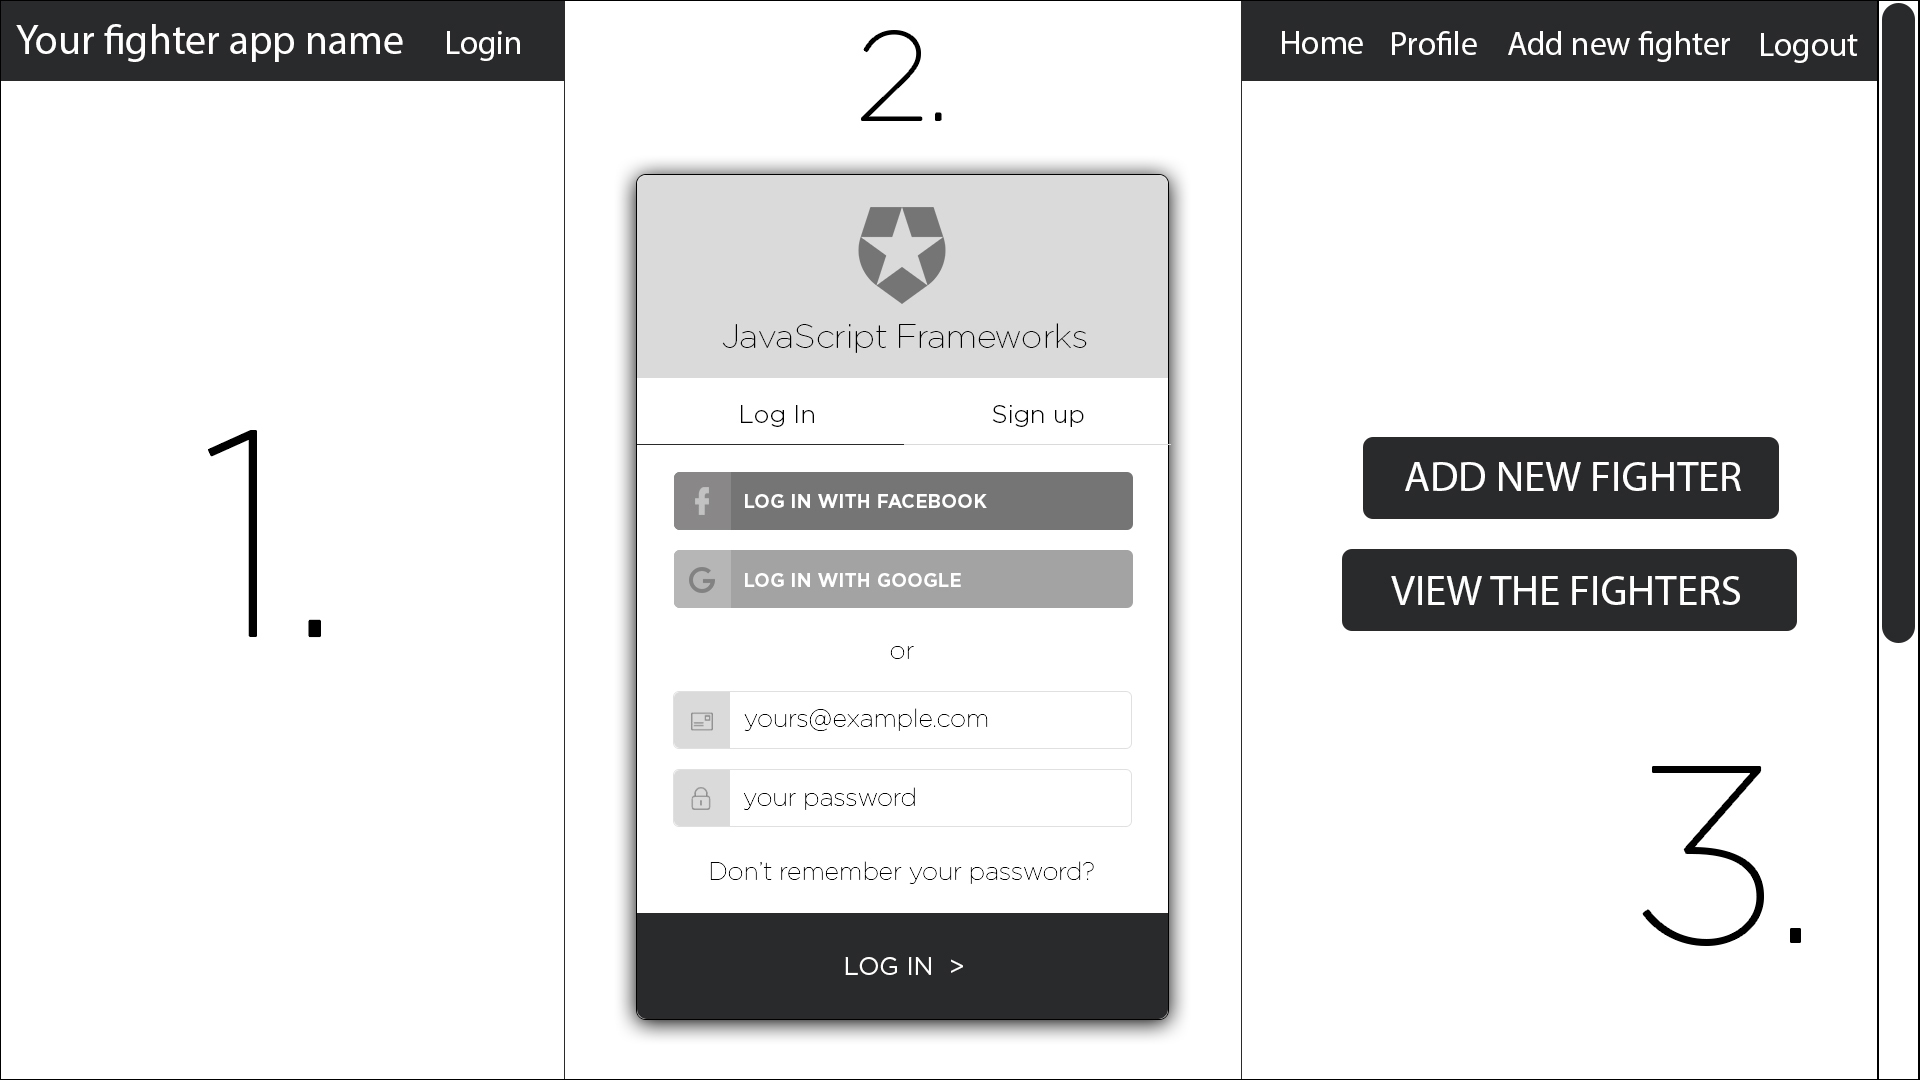
\includegraphics[scale=0.7]{kepek/login_auth0_home.jpg}
\caption{Főoldal (Home)}
\label{fig:home}
\end{figure}

A VIEW THE FIGHTERS feliratú linkre kattintva a /fighters oldal jelenítődik meg a harcosok listájával (\ref{fig:search_bar}. ábra).

\begin{figure}[htb]
\centering
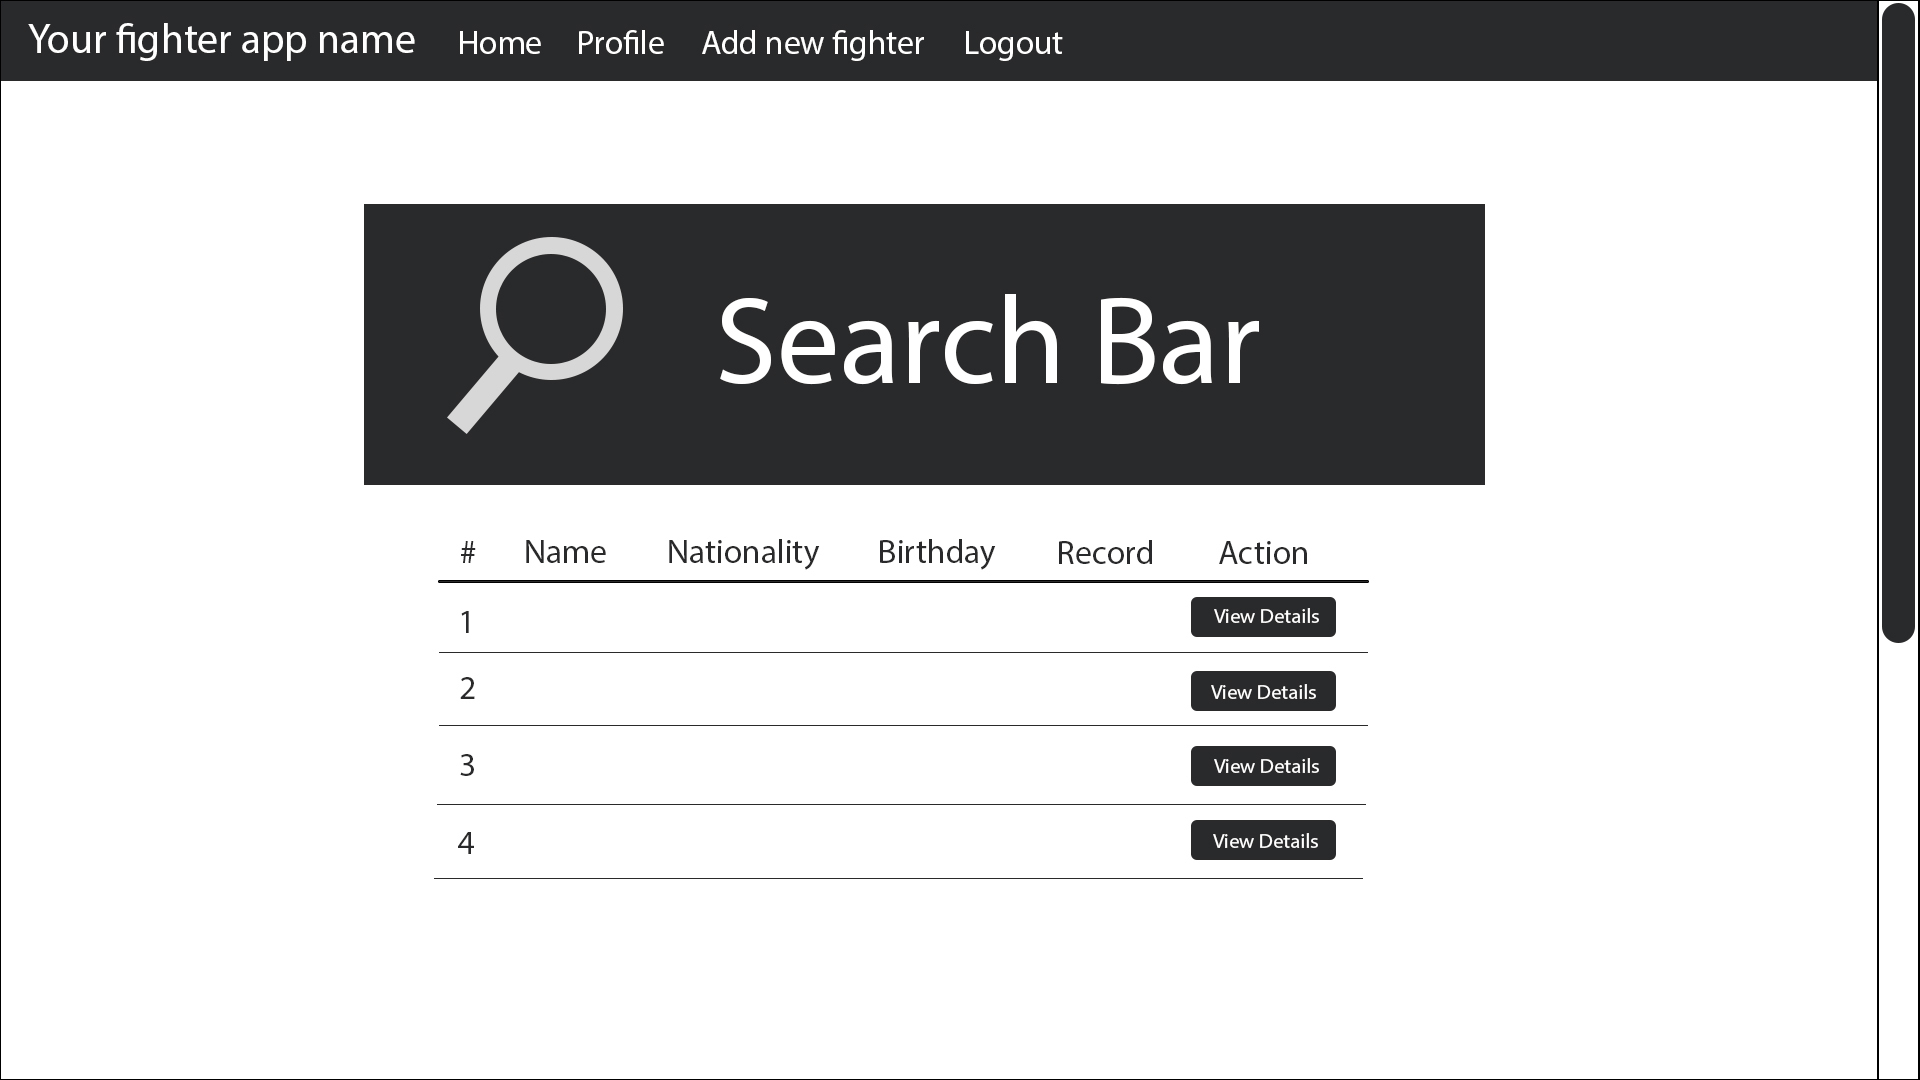
\includegraphics[scale=0.7]{kepek/search_bar.jpg}
\caption{Harcos lista oldal (Fighters)}
\label{fig:search_bar}
\end{figure}

\begin{figure}[htb]
\centering
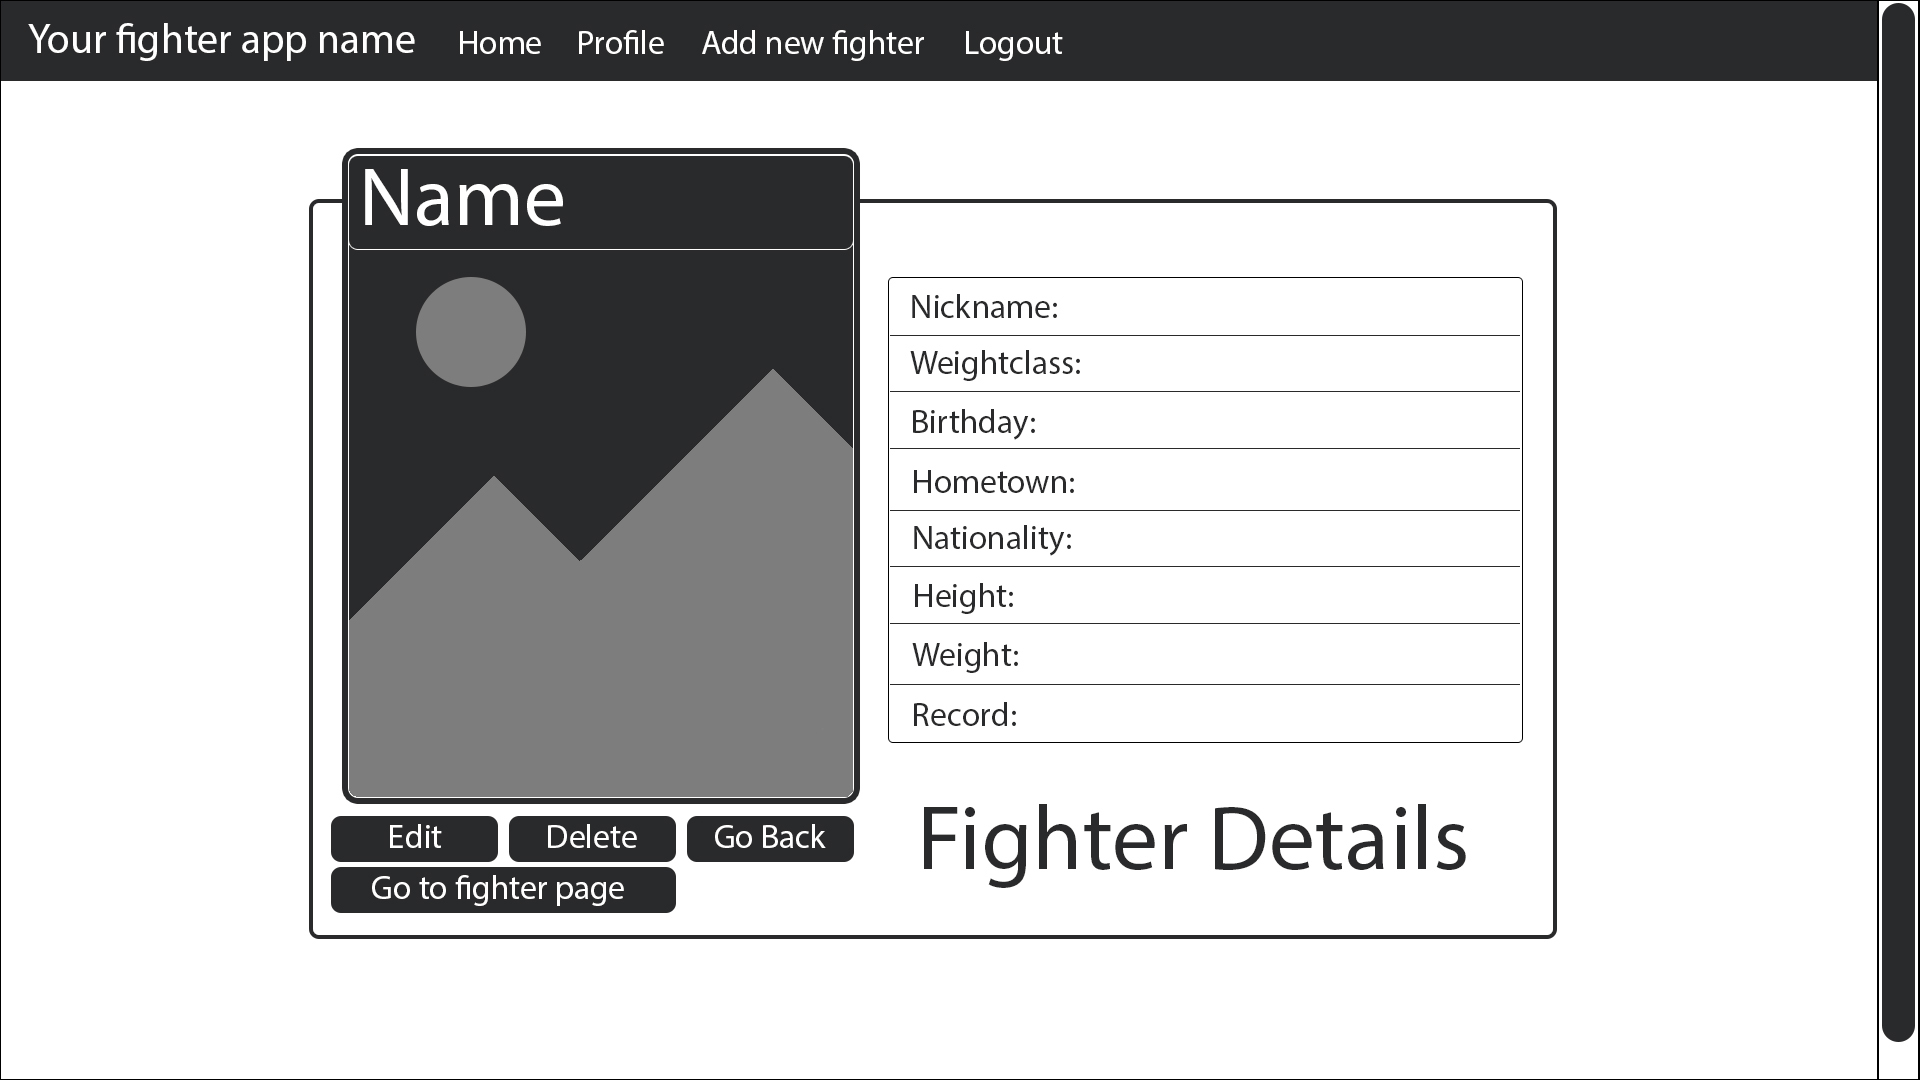
\includegraphics[scale=0.7]{kepek/details.jpg}
\caption{Harcos adatait megjelenítő oldal (Fighter Details)}
\label{fig:details}
\end{figure}

A harcos sorában lévő View Details feliratú linkre kattintva az adott harcos adatait tartalmazó oldal jön be /fighters/details/id formában (\ref{fig:details}. ábra).

A details oldalon az "Edit" gombra kattintva a program átirányítja a felhasználót a /fighters/edit/:id oldalra, ahol a harcos adatait tudja frissíteni (\ref{fig:edit}. ábra).

\begin{figure}[htb]
\centering
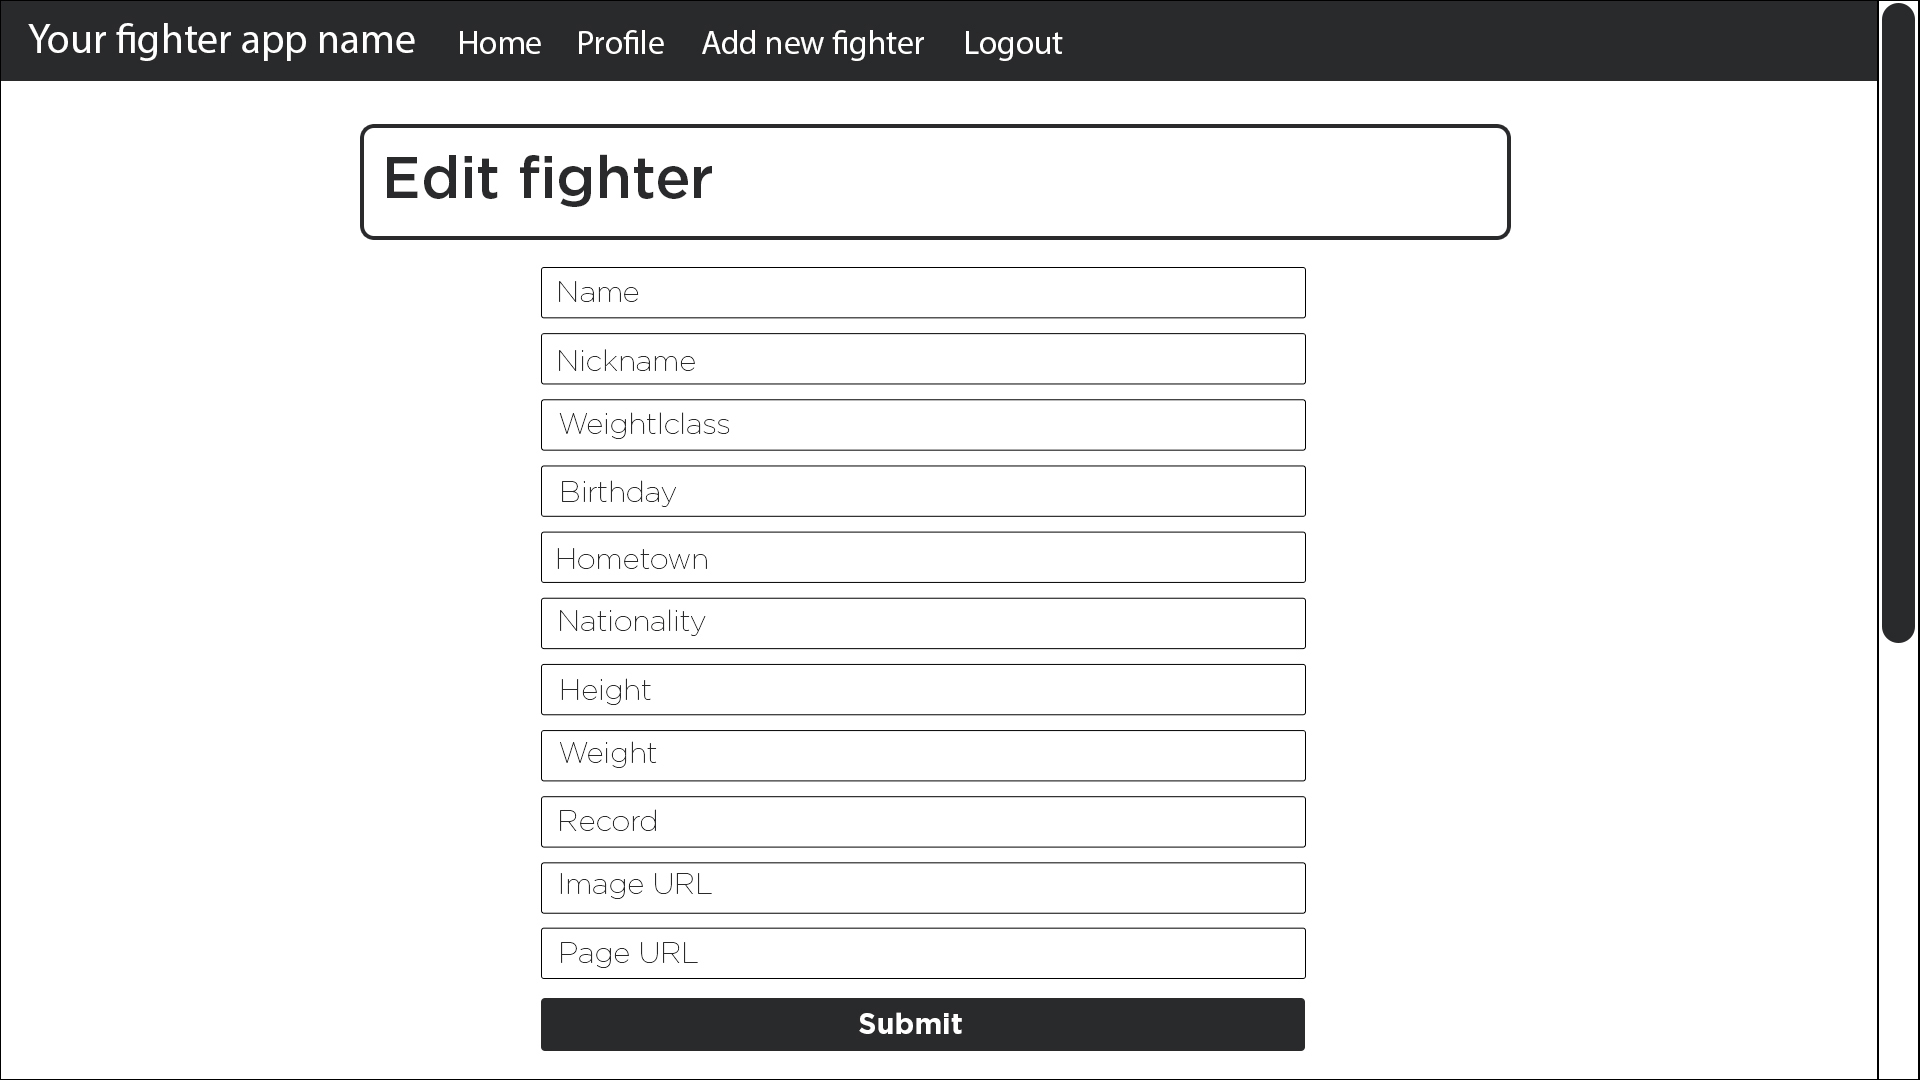
\includegraphics[scale=0.7]{kepek/edit_fighter.jpg}
\caption{Harcos adatait változtató oldal (Edit Fighter Details)}
\label{fig:edit}
\end{figure}

\begin{figure}[htb]
\centering
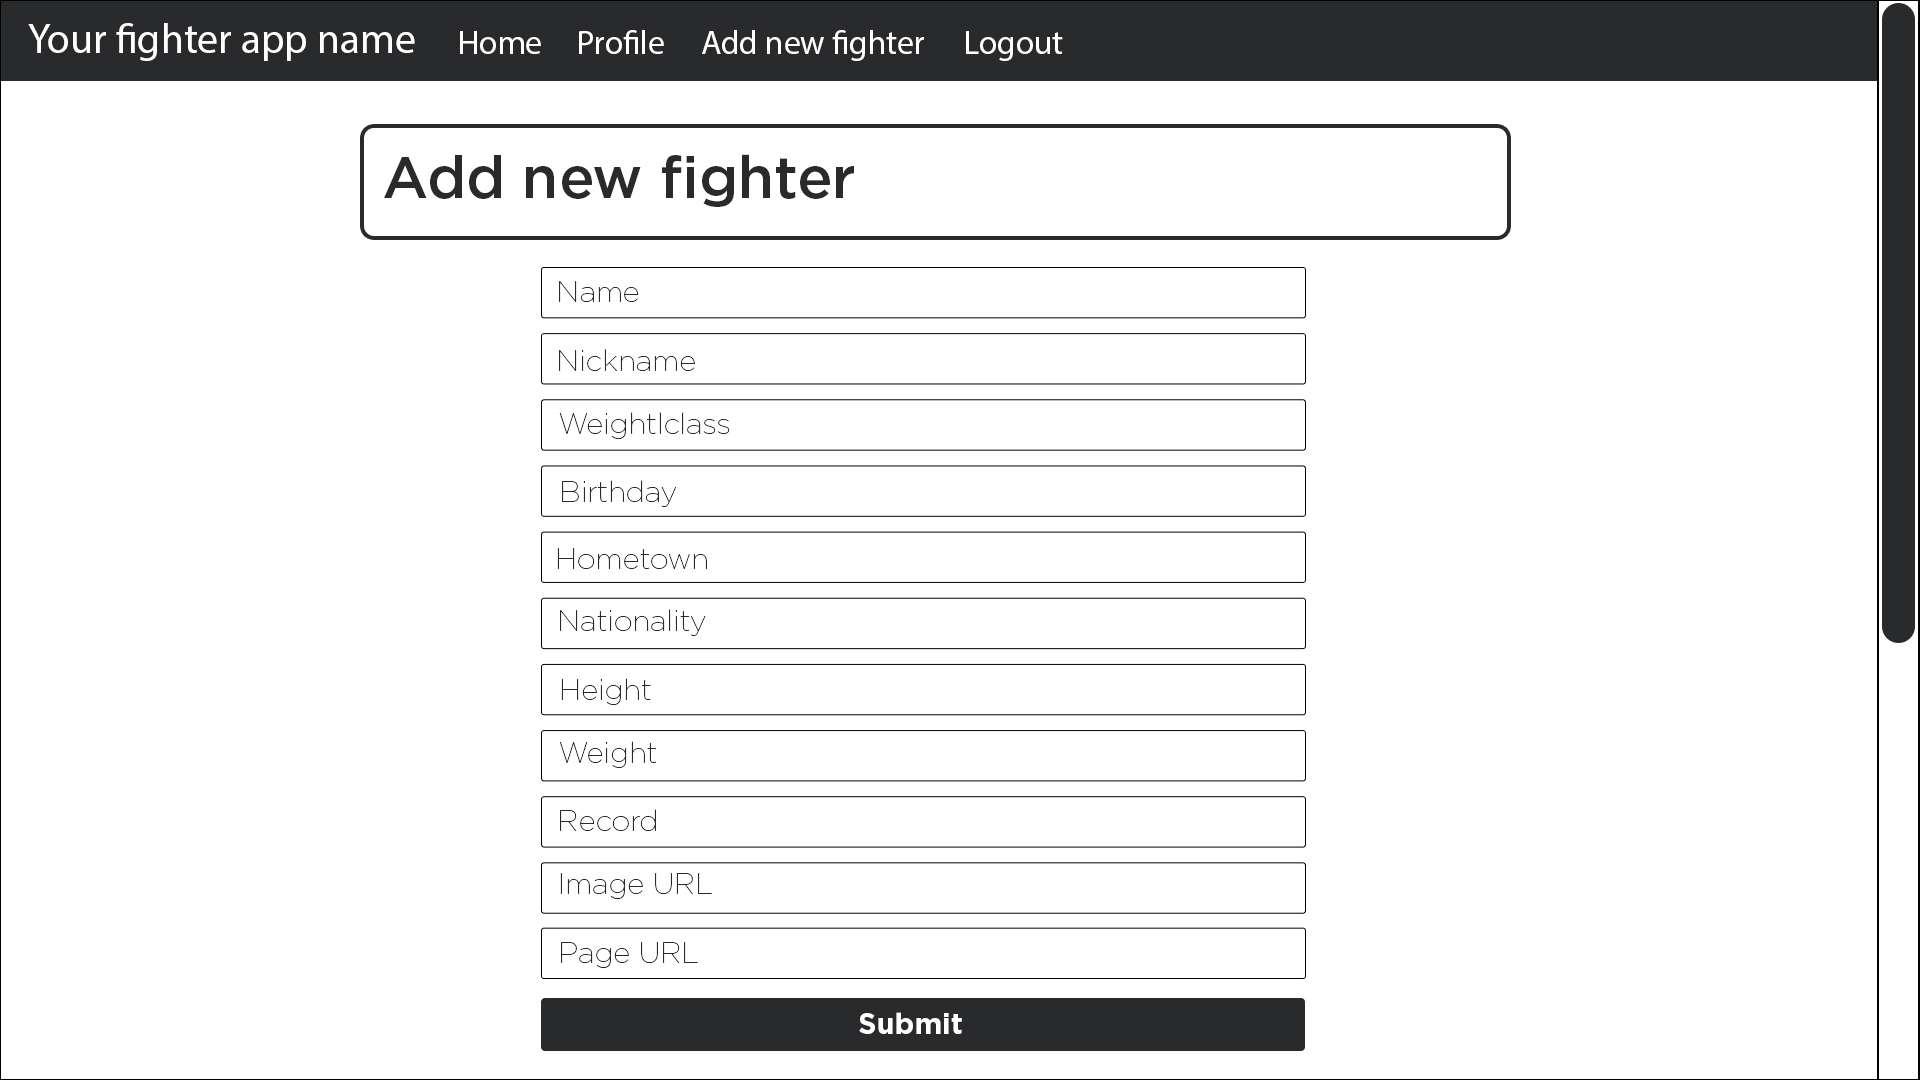
\includegraphics[scale=0.7]{kepek/add_new_fighter.jpg}
\caption{Új harcost létrehozó oldal (Add new fighter)}
\label{fig:add}
\end{figure}
\newpage
Végül ha a felhasználó bejelentkezés után (\ref{fig:home}. ábra), az ADD NEW FIGHTER feliratú gombra kattint, akkor a /fighters/add oldal ugrik fel (\ref{fig:add}. ábra).

\Chapter{AngularJS implementáció}

CRUD műveletek megvalósítása: (CREATE, READ, UPDATE, DELETE) – Létrehozás, Lekérés, Frissítés, Törlés
Az web alkalmazásban ezeket a funkciókat a MMA harcosokon lehet végrehajtani.

A szerver által nyújtott REST API megvalósítása biztosítja a kód működőképességét.

A harcosokon végzett műveleteket a fighters.js nevű fájl tartalmazza.

Ahhoz, hogy minden megfelelően működjön létre kell hozni egy modult az alkalmazásban:

\begin{cpp}
var app = angular.module('app');
\end{cpp}

Ezután egy hozzátartozó kontrollert:

\begin{cpp}
app.controller('FightersController', ['$scope', '$http', '$location', 
'$stateParams',  '$state', function($scope, $http, $location, 
$stateParams, $state){
}]);
\end{cpp}

Ebbe a kontrollerbe tehetjük be a különböző funkciókat: A harcosok szerverről való lekérése:

\begin{cpp}
$scope.getFighters = function(){
$http({
	method: 'GET',
	url: '/api/fighters'
	}).then(function successCallback(response) {
	$scope.fighters = response.data;
	}, function errorCallback(response) {
});}
\end{cpp}

Ehhez egy GET kérést szükséges elküldeni a szervernek, ami visszaküldi egy response objektumban ez esetben a fighters objektumot, ami a harcosok adatait tartalmazza.

A /api/fighters URL-en lévő adatokat adja vissza, amik JSON formátumban vannak eltárolva.

A következő példakód egy harcos hozzáadását mutatja be, ehhez egy POST HTTP kérés elküldésére van szükségünk:

\begin{cpp}
$scope.addFighter = function(){
		console.log($scope.fighter);
		$http({
			method: 'POST',
			url: '/api/fighters/',
			data: $scope.fighter
		}).then(function successCallback(response) {
			$state.go("fighters");
		}, function errorCallback(response) {
  		});
	}
\end{cpp}

Miután a szerver sikeresen teljesítette a kérést, a \texttt{\$state.go("fighters");} kódsor
visszairányítja a felhasználót a ’fighters’ nevű route-ra, ami a /fighters oldallal egyezik meg.

Egy harcos adatainak frissítéséhez már szükség van a frissíteni kívánt harcos szerveren tárolt id mezőjére.

\begin{cpp}
$scope.updateFighter = function(){
		var id = $stateParams.id;
		$http({
			method: 'PUT',
			url: '/api/fighters/' +id,
			data: $scope.fighter
		}).then(function successCallback(response) {
			$state.go("fighters");
		}, function errorCallback(response) {
  		});
	} 
\end{cpp}

Ezt egy változó létrehozásával tehetjük meg, amiben letároljuk az id-t a 
\texttt{\$stateParams} segítségével, ami az URL-ből olvassa ki az id-t. Sikeres végrehajtás után a szerver ismét visszairányít a ’fighters’ nevű route-ra, tehát a /fighters oldalra, hogy lássuk a végrehajtott változtatásokat.

Egy harcos törléséhez szintén szükségünk van az id-jére, amit a megfelelő HTML oldalon lévő törlés gombnál adunk meg neki, ami a megfelelő harcos id-jével hívja meg a removeFighter nevű függvényt.

\begin{cpp}
$scope.removeFighter = function(id){
		$http({
			method: 'DELETE',
			url: '/api/fighters/' +id,
			data: $scope.fighter
		}).then(function successCallback(response) {
			$state.go("fighters");
		}, function errorCallback(response) {
  		});
	}
\end{cpp}

A következő funkció a harcosok táblázatának betűsorozatra való leszűkítése. Ekkor, ha a felhasználó egy kereső mezőbe begépel egy betűt, vagy betűsorozatot, amit az egyik, vagy több harcos neve tartalmaz, akkor a táblázat, ami megjeleníti a harcosokat dinamikusan szűkül le, és mutatja azt, vagy azokat a harcosokat, akinek, vagy akiknek a nevére illik a keresőmező tartalma.

\begin{cpp}
<div id="search">
  <input type="text" ng-model="search.name" 
  placeholder="Search fighters..."/>
</div>
\end{cpp}

Az kereső mezőn kívül szükség van egy filterre is, amit a \texttt{<table>} \texttt{<tbody>} részének első sorába írhatunk be: ez jeleníti meg az egyes harcosok nevét, becenevét, és egy View Details feliratú linket, amire kattintva megtekinthetők az adott harcos adatai.

\begin{cpp}
<tbody>
	<tr ng-repeat="fighter in fighters | filter:search">
		<td>{{ fighter.name }}</td>
        <td>{{ fighter.nickname }}</td>
	</tr>
</tbody>
\end{cpp}

\Section{Form validáció}

A form validáció többféle módon valósítható meg.
Az egyik megvalósítási lehetőség a \texttt{\$valid} és \texttt{\$invalid} state-ekkel (állapot):

\begin{cpp}
<form name="fighterForm" ng-submit="addFighter(fighterForm.$valid)" 
novalidate>
\end{cpp}

A novalidate kulcsszó ahhoz szükséges, hogy kikapcsoljuk a HTML5 alapvető validációs funkcióját.

\begin{cpp}
<button type="submit" ng-disabled="fighterForm.$invalid" 
		class="btn btn-default">Submit</button>
\end{cpp}

Ha a form még nem érvényes (valid) akkor a Submit (elküldés) gombra való kattintás letiltásra kerül, így a felhasználó nem tudja elküldeni a form-ot.

Szöveg mezők validációját a következőképpen valósítottam meg:

\begin{cpp}
<div class="form-group" ng-class="{ 'has-error' : 
fighterForm.name.$touched && !fighterForm.name.$dirty || 
fighterForm.name.$invalid && !fighterForm.name.$pristine }">
<label>Name*</label>
<input type="text" class="form-control" name="name" 
ng-model="fighter.name" placeholder="Name" ng-minlength="3" required/>
<p ng-show="fighterForm.name.$touched && !fighterForm.name.$dirty && 
!fighterForm.name.$error.minlength || fighterForm.name.$invalid && 
!fighterForm.name.$pristine && !fighterForm.name.$error.minlength" 
class="help-block">Name is required.</p>
<p ng-show="fighterForm.name.$error.minlength" class="help-block">
    Name is too short.</p>
</div>
\end{cpp}

Az alkalmazás akkor írja ki a validációs hibaüzenet, ha egyszerre teljesülnek az alábbi feltételek:
\begin{itemize}
\item az input mezőbe kattint a felhasználó, de nem ír a mezőbe semmit 
\item vagy ha a mező értéke nem érvényes, pedig már írt bele
\end{itemize}

A hibaüzenet a mezőből való kikattintás után jelenik meg. A név mező kötelező hibaüzenet (Name is required.) csak abban az esetben jelenik meg, ha a mező üres, tehát a minimum karakterszám nem teljesülése még nem lehet hiba.

Amint a felhasználó beleír valamit a mezőbe, a „Name is required” hibaüzenet eltűnik és a Név túl rövid (Name is too short.) hibaüzenet jelenik meg egészen addig, amíg a név mező karaktereinek száma el nem éri a 3-at.

A has-error ng-class (AngularJS osztály) hiba esetén a hibaüzenetnek piros színnel és a beviteli mezőnek piros szegéllyel való megjelenítéséért felelős.

A szám mezőknél a min és max direktívákat használtam:

\begin{cpp}
<label>Height*</label>
<input type="number" class="form-control" name="height" 
ng-model="fighter.height" placeholder="Height" min="155" max="205" 
required/>
\end{cpp}

Az előző példához hasonlóan a „Height is required” hibaüzenet nem jelenik meg, csak üres mező esetében. Ezután, ha a beírt számérték nem 155 és 205 közé esik, akkor a 
„Height value must be between 155 and 205 cm.” hibaüzenet jelenik meg.

A record mezőnél az ng-pattern direktívával szűkítettem le a lehetséges megadható eseteket:

\begin{cpp}
<label>Record*</label>
<input type="text" class="form-control" name="record" 
ng-model="fighter.record" placeholder="Record" 
ng-pattern="/^[0-9]{1,2}-[0-99]{1,2}-[0-99]{1,2}$/" required/>
\end{cpp}

Ezzel elérhető, hogy csak akkor legyen érvényes a record mező értéke, ha az [0-999]-[0-999]-[0-999] formátumú. Ezt a mezőt is kötelező kitölteni így itt is csak akkor jelenik meg a „Record is required” hibaüzenet, ha még nem írt a felhasználó a mezőbe.

Ezután ha nem a fent említett formátumban írt a felhasználó a mezőbe, akkor a „The record must be in Wins-Draws-Losses form.” hibaüzenet jelenik meg, ami azt jelenti, hogy a rekord mezőt győzelem-döntetlen-vereség formában kell kitölteni, például: 30-2-3.

Az image\_url-hez hozzáadott
\begin{cpp}
ng-pattern="/^https?://.+$/"
\end{cpp}
direktívával pedig a harcos avatarjának URL link validációját készítettem el, ami ha a felhasználó nem http:// vagy https://-el kezdődő URL címet ad meg, akkor „Image URL must be valid.” hibaüzenetet kap.

\Section{Routing}

Az oldalak közötti routing az ui.router szervízzel van megoldva.
Ehhez az angular module-ba meg kell adnunk az ui.router-t, mint függőséget (dependency).

\begin{cpp}
angular
    .module('app', ['ui.router']);
\end{cpp}

Az alábbi kód /fighters oldal megjelenítését biztosítja, a FightersController biztosítja a funkciókat, a /fighters oldalra való navigációkor pedig az alkalmazás a fighters.html template-t tölti be.

\begin{cpp}
$stateProvider
.state('fighters', {
        url: '/fighters',
        controller: 'FightersController',
        templateUrl: 'app/views/fighters.html',
        controllerAs: 'vm' });
\end{cpp}

\Section{Projekt struktúra}

\begin{figure}[htb]
\centering
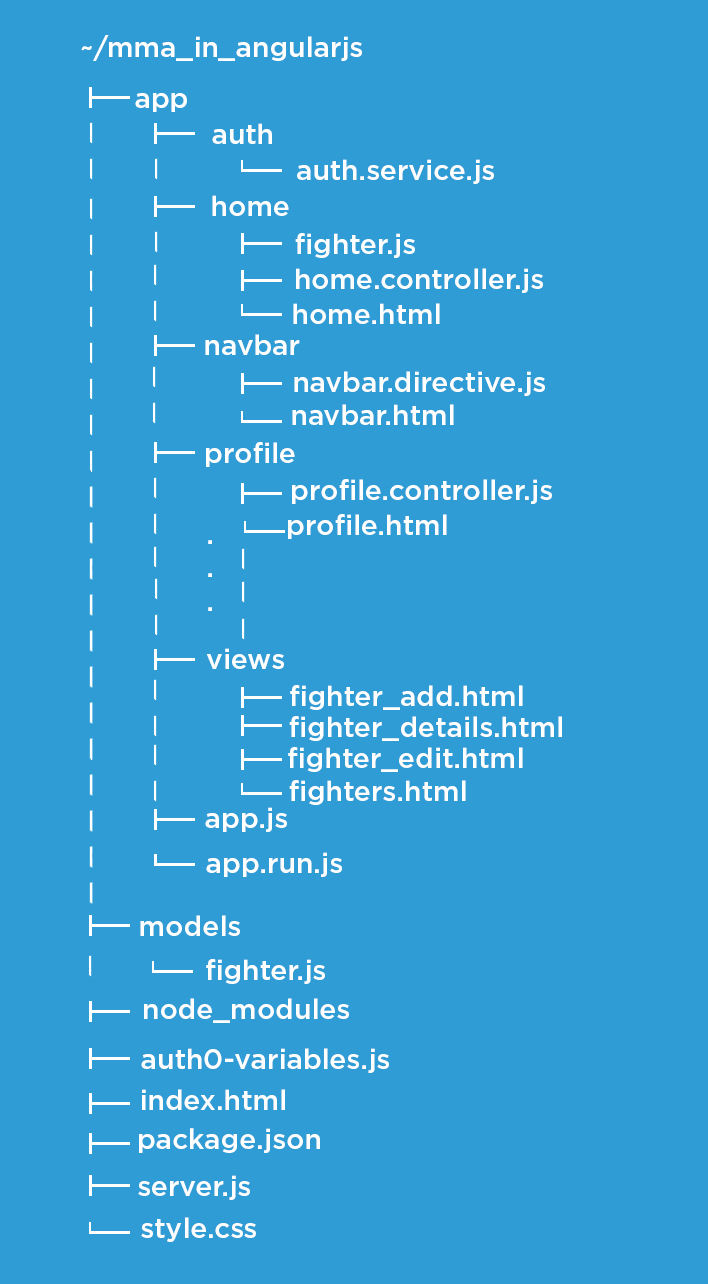
\includegraphics[scale=0.8]{kepek/mma_in_angularjs.jpeg}
\caption{Az AngularJS projekt struktúrája}
\label{fig:angularjs_structure}
\end{figure}

\Chapter{Angular2 implementáció}

CRUD műveletek: A műveletek megvalósításához szükséges funkciókat a szervíz tartalmazza, ebben az esetben a FighterService.

\begin{cpp}
@Injectable()
export class FighterService {
  constructor(private http: Http) { }
  getAllFighters() {
    return new Promise((resolve, reject) => {
      this.http.get('/fighter')
        .map(res => res.json())
        .subscribe(res => {
          resolve(res);
        }, (err) => {
          reject(err);
        });
    });  }  }
\end{cpp}

A getAllFighters() GET kérést küld a szervernek. Ennek a függvénynek a segítségével kérhetők le az eltárolt harcosok.
Egy harcos adatainak frissítésére szolgáló függvény az 

\begin{cpp}
updateFighter(id, data) {
    return new Promise((resolve, reject) => {
        this.http.put('/fighter/'+id, data)
          .map(res => res.json())
          .subscribe(res => {
            resolve(res);
          }, (err) => {
            reject(err);
          });
    });
  }
\end{cpp}

A HTML oldalakat külön komponensek vezérlik:

Ezeket a komponenseket az „ng g component komponensnév” paranccsal lehet létrehozni, ami automatikus legenerálja a szükséges fájlokat és hozzáadja az új komponenst az app.module.ts fájlhoz.

\begin{cpp}
@Component({
  selector: 'app-fighter',
  templateUrl: './fighter.component.html',
  styleUrls: ['./fighter.component.css']
})
export class FighterComponent implements OnInit {
  fighters: any;
  constructor(private fighterService: FighterService) { }
  ngOnInit() {
    this.getFighterList();
  }
  getFighterList() {
    this.fighterService.getAllFighters().then((res) => {
      this.fighters = res;
    }, (err) => {
      console.log(err);
    });}}
\end{cpp}

A „fighters” oldal, ami a harcosok megjelenítésére szolgál egy komponens, a hozzátartozó template-t a templateUrl kifejezéssel tudjuk megadni. A kinézetét a megfelelő nevű .css kiterjesztésű fájl tartalmazza, amit a styleUrls kifejezéssel adhatunk meg.

Ez az oldal a getFighterList() nevű függvény használatával kéri le a szerveren tárolt harcosokat.

A harcosok táblázatának keresőmezővel való szűrése:
A harcosok táblázatának szűréséhez egy pipe-ra van szükségünk:

\begin{cpp}
export class FilterPipe implements PipeTransform {
  transform(fighters: any, search: any): any {
    if (search === undefined) return fighters;
    return fighters.filter(function(fighter){
    	return fighter.name.includes(search);  })}}
\end{cpp}

Ezenkívül szükség van még egy kereső mezőre: 

\begin{cpp}
<input type="text" [(ngModel)]="search" 
placeholder="Search fighters..."/>
\end{cpp}

Használata a | filter:szűrőmező neve paranccsal lehetséges:

\begin{cpp}
<tbody>
      <tr *ngFor="let fighter of fighters | filter:search">
        <td>{{ fighter.name }}</td>
        <td>{{ fighter.nickname }}</td>
      </tr>
    </tbody>
\end{cpp}

Továbbá egy import-ra, amit az app.module.ts fájlhoz kell hozzáadnunk:

\begin{cpp}
import { FilterPipe } from './filter.pipe';
\end{cpp}

Majd ugyanebben a fájlban az @NgModule declarations részéhez hozzá kell adni a FilterPipe osztályt.

\begin{cpp}
@NgModule({
  declarations: [
    AppComponent,
    HomeComponent,
    FighterComponent,
    FilterPipe
\end{cpp}

\Section{Routing}

A routing-hoz szükség van a

\begin{cpp}
import { RouterModule } from '@angular/router';
\end{cpp}

sorra, amit az app.module.ts nevű fájlban kell megadnunk.
Ezenkívül szükség van még az app.component.html fájlban a <router-outlet></router-outlet> tag-okra.

Route-k (útvonalak) megadása az app.routes.ts fájlban és az 

\begin{cpp}
import { ROUTES } from './app.routes'; 
\end{cpp}

sorra az app.module.ts fájlban.

\begin{cpp}
export const ROUTES: Routes = [
  { path: ' ', component: HomeComponent },
  { path: 'fighters', component: FighterComponent },
  { path: '**', redirectTo: ' ' }
];
\end{cpp}

Ez a kódrészlet azt mutatja be, hogy ha a felhasználó az URL-ben nem ír be semmit a / jel után, akkor az alkalmazás a HomeComponent nevű komponens kapja meg a vezérlést, ami a home.component.html nevű fájlt tölti be.

\begin{cpp}
@Component({
  selector: 'app-home',
  templateUrl: './home.component.html',
  styleUrls: ['./home.component.css']
})
\end{cpp}

A /fighters oldal pedig a FighterComponent-ben meghatározott templateUrl-t és styleUrls-t tölti be.

A lapok közötti navigálás linkekkel történik: 
A /fighter-create oldalról a /fighters oldalra való visszalépés esetén:

\begin{cpp}
<a [routerLink]="['/fighters']">Go back</a>
\end{cpp}

\Section{Form validáció}

A form validációnál a disabled-re (letiltott) állítottam a Submit gombot:

\begin{cpp}
<button type="submit" class="btn btn-success" 
[disabled]="!fighterForm.form.valid">Submit</button>
\end{cpp}

Így ha a fighterForm nevű űrlap (form) nem valid, akkor a Submit gomb ki van kapcsolva.

Mezők validálása az Angular 2 által biztosított direktívákkal történik:

\begin{cpp}
<form (ngSubmit)="saveFighter()" #fighterForm="ngForm">
\end{cpp}

A form fejlécében meg kell adni a form nevét, ez esetben „fighterForm”.

Majd a Submit gomb letiltása a [disabled]="!fighterForm.form.valid" sor Submit button-hoz való hozzáadásával érhető el, ami letiltja a gombot, ha a fighterForm nevű form nem érvényes (valid).

\begin{cpp}
<button type="submit" class="btn btn-success" 
[disabled]="!fighterForm.form.valid">Submit</button>
\end{cpp}

A name mező validálásához meg kell adni a kívánt direktívákat, ebben az esetben, hogy a mező kitöltésekor minimum 3 karakter hosszúságú nevet kell beírnia a felhasználónak. (minlength=”3”)

A „required” jelző pedig a mező kitöltését követeli meg a felhasználótól.

\begin{cpp}
<label for="name">Name*</label>
<input type="text" class="form-control" [(ngModel)]="fighter.name" 
name="name" id="name" #name="ngModel" required minlength="3">
<div *ngIf="name.errors && (name.dirty || name.touched)" 
	class="alert alert-danger">
	<div [hidden]="!name.errors.required">
    	Name is required!
    </div>
    <div [hidden]="!name.errors.minlength">
    	Name must be at least 3 characters long.
    </div>
</div>
\end{cpp}

Ha a name mező hibás és már írtak bele, vagy csak belekattintottak, akkor a mező alatt megjelenítődik az épp aktuális hibaüzenet.

A record mező validálásához pattern-t kell hozzáadni a mezőhöz:

\begin{cpp}
<label for="record">Record*</label>
<input type="text" class="form-control" [(ngModel)]="fighter.record" 
name="record" id="record" #record="ngModel" 
pattern="[0-9]{1,2}-[0-9]{1,2}-[0-9]{1,2}" required>
<div *ngIf="record.errors && (record.dirty || record.touched)" 
class="alert alert-danger">
<div [hidden]="!record.errors.required">
	Record is required!</div>
<div [hidden]="!record.errors.pattern">The record must be in 
Wins-Draws-Losses form.</div></div>
\end{cpp}

Ha a beírt adatok nem egyeznek meg a pattern-nel, akkor a felhasználó a „The record must be in Wins-Draws-Losses form.” hibaüzenetet kapja.

A harcos avatarjának image\_url mezőben megadott URL linkhez tartozó validációnál itt is a pattern="https?://.+" direktívát kell a beviteli mezőhöz hozzáadni, ezután, ha a felhasználó az Image URL linket nem a megfelelő formában adja meg, az „Image URL must be valid!” hibaüzenetet kapja.
\newpage

\Section{Projekt struktúra}

\begin{figure}[htb]
\centering
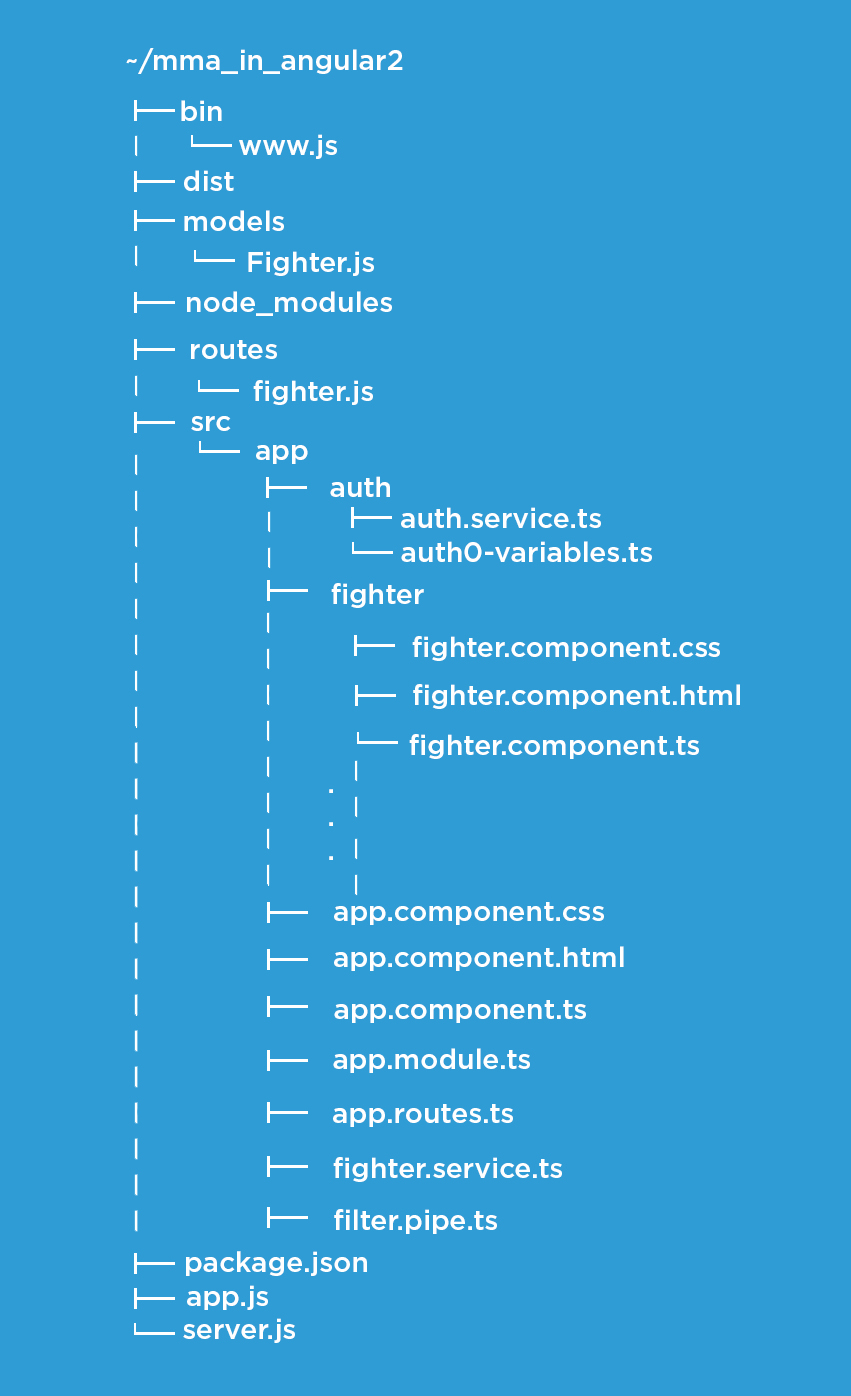
\includegraphics[scale=0.7]{kepek/mma_in_angular2.jpeg}
\caption{Az Angular2 projekt struktúrája}
\label{fig:angularjs_structure}
\end{figure}

\Chapter{VueJS implementáció}

CRUD műveletek megvalósítása a services/FightersService.js fájlban:

\begin{cpp}
export default {
  fetchFighters () {
    return Api().get('fighters')
  }, 
  addFighter (params) {
    return Api().post('fighters', params)
  },
  updateFighter (params) {
    return Api().put('fighters/' + params.id, params)
  },
  getFighter (params) {
    return Api().get('fighter/' + params.id)
  },
  deleteFighter (id) {
    return Api().delete('fighters/' + id)
    this.fetchFighters();
  }
}
\end{cpp}

A "fetchFighters" nevű függvény visszaadja az Api().get(’fighters’) kérést, amit az "axios" modul végez el, ami egy promise alapú http kliens. Ehhez szükséges importálni a "FightersService.js" fájlban a services/Api.js fájlt, ami biztosítja az axios modult.

\begin{cpp}
import Api from '@/services/Api'
\end{cpp}

A "getFighter()" és az "updateFighter()" függvények az URL címből veszik át a harcos id-jét.

A "deleteFighter()" függvény miután megkapta az id-t, meghívja a "fetchFighters()" nevű függvényt, ami újra lekéri az aktuálisan eltárolt harcosokat.

Api.js fájl tartalma:

\begin{cpp}
import axios from 'axios'
export default() => {

  return axios.create({
    baseURL: `http://localhost:8081`
  })
}
\end{cpp}

\Section{Routing}

A routing-hoz szükséges importálni és használni a "vue-router"-t:

\begin{cpp}
import Router from 'vue-router'
\end{cpp}

A routing-ok (útvonalak) létrehozásánál a Vue.use(Router) sorral adjuk meg, hogy a program használja Router-ként a beimportált "vue-router" nevű modult.

\begin{cpp}
export default new Router({
mode: 'history',
  routes: [
{
      path: '/fighters',
      name: 'Fighters',
      component: Fighters
  },
  {
      path: '/fighters/new',
      name: 'NewFighter',
      component: NewFighter  }]})
\end{cpp}

Az alapvető beállítás a "vue-router" modulban az úgynevezett "hash mode", ami az URL hash-t (\#) használja a teljes URL cím reprezentálására, így ha az URL változik, az oldal nem fog újra lefrissülni.

A mode: ’history’ használatával a vue-router-t "history mode"-ban használhatjuk, amivel megszabadulhatunk a hash-től az URL címekben. Ez a mód az history.pushState API használatával megteremti annak a lehetőségét, hogy a felhasználó navigálhasson az URL-ek között, anélkül, hogy az oldal újra lefrissülne. Ehhez megfelelő szerver konfiguráció szükséges, különben a felhasználó egyes oldalak elérésekor 404-es hibaüzenetet kaphat.

A path definiálja az oldal URL címét, a component mutatja meg, hogy melyik .vue fájl tartalmát kell megjeleníteni az URL-re való látogatáskor. Ehhez a megadott komponenseket importálnunk kell.

\begin{cpp}
import Fighters from '@/components/Fighters'
import NewFighter from '@/components/NewFighter'
\end{cpp}

A /fighters/new URL megnyitásakor a NewFighter.vue komponens töltődik be, ami tartalmazza a megjelenítendő template-t, amiben egy új harcos létrehozásához szükséges form található.

\Section{Form validáció}

A form validálás többféle módon történhet, az egyik ilyen a "vee-validate" modul használatával történő validáció, amelyhez először telepíteni kell a modult az npm csomagkezelő vagy CDN segítségével, majd az alábbiakat kell importálni az alkalmazáshoz tartozó "main.js" fájlban:

\begin{cpp}
npm install vee-validate --save
import Vue from 'vue'
import VeeValidate from 'vee-validate'
Vue.use(VeeValidate)
\end{cpp}

A name mező validálása:

\begin{cpp}
<div class="form-group" :class="{'has-error': errors.has('name') }">
<label for="Name">Name*</label>
<input type="text" v-model="name" name="name" class="form-control" 
   	id="Name" placeholder="Name" 
   	v-validate="'required|alpha_spaces|min:3'"> 
	<span v-show="errors.has('name')" class="text-danger">
	{{ errors.first('name') }}</span>
</div>
\end{cpp}

A "v-validate" input mezőhöz való hozzáadása után lehet megadni az úgynevezett szabályokat (rules), ez esetben required, alpha\_spaces és min:3, tehát a mező kitöltése kötelező, a felhasználónak csak alfabetikus karaktereket és közöket (space) lehet a mezőbe írnia, egyéb esetben a mező nem érvényes. A min:3 a minimum karakterszámot állítja be háromra.

A "v-show" direktíva használatával piros színű szegéllyel határolt mező jelenik meg, ha a mező értéke még nem valid (érvényes). Ha a felhasználó belekattint a mezőbe, majd kikattint belőle úgy, hogy nem írt a mezőbe semmit, akkor a program által előre definiált hibaüzenet jelenik meg: "The name field is required".

Ezenkívül minden egyes szabályra is az előre meghatározott hibaüzenetek jelennek meg, ha a felhasználó numerikus karaktert ír be, vagy ha kevesebb, mint három karakter a begépelt szöveg hossza.

A szám mezők validációja hasonlóan történik:

\begin{cpp}
<div class="form-group" :class="{'has-error': errors.has('height') }">
	<label for="Height">Height*</label>
	<input type="number" class="form-control" name="height" 
	placeholder="Height" v-model="height" id="Height" 
	v-validate="'required|min_value:155|max_value:205'">
	<span v-show="errors.has('height')" class="text-danger">
	{{ errors.first('height') }}</span>
</div>
\end{cpp}

Itt a "height" mező értékét adhatjuk meg a min\_value és max\_value szabályokkal, ha a felhasználó nem 155 és 205 közötti számértéket ír be a mezőbe, akkor megjelenik a hibaüzenet.

A "record" mező a
\begin{cpp}
v-validate="'required|regex:^[0-9]+[-][0-9]+[-][0-9]+$'"
\end{cpp}
megadása után csak akkor lesz érvényes, ha a felhasználó azt ilyen formában adja meg. Például: 100-10-1

Az "image\_url" mezőnél pedig a
\begin{cpp}
v-validate="'required|regex:^https?://.+$'"
\end{cpp}
megadása után a felhasználó csak érvényes URL linket adhat meg a harcos avatarjának.

A form fejlécében lévő @submit.prevent=”validateBeforeSubmit” arra szolgál, hogy mikor a felhasználó rákattint a "Submit" gombra, a form-ot a program még nem küldi el, csak miután meghívta a "validateBeforeSubmit()" nevű függvényt.

\begin{cpp}
<form @submit.prevent="validateBeforeSubmit">
\end{cpp}

\begin{cpp}
validateBeforeSubmit() {
      this.$validator.validateAll().then((result) => {
        if (result) {
          // eslint-disable-next-line
          this.addFighter()
          return; }});
}
\end{cpp}

Ez a függvény megnézi a "validateAll()" függvény eredményét, és ha minden mező érvényes, akkor meghívja az "addFighter()" függvényt, ami a "FightersService" szervízben van definiálva. Ekkor, ha a felhasználó a "Submit" gombra kattint, az összes hibaüzenet azonnal megjelenik, de az "addFighter()" függvény még nem hívódik meg.

A "NewFighter" komponens tartalmaz egy <template></template> tag-ok közötti kódrészletet, amiben a megjelenítendő template-t tudjuk megadni. 

A <script></script> tag-ok között adhatjuk meg a szükséges függvényeket, metódusokat, funkciókat.

Ehhez importálnunk kell a FighterService-t:

\begin{cpp}
import FightersService from '@/services/FightersService'

export default {
  name: 'NewFighter',
  data () {
    return {
      name: ' ',
      nickname: ' ' }}
\end{cpp}

A "data" részben a form-ból átvett mezőknek az értékét állítjuk be egy üres sztring-re.
Majd a "methods" résznél megadjuk, hogy a FighterService-ben lévő "addFighter()" függvény pontosan mit hajtson végre:

\begin{cpp}
methods: {
    async addFighter () {
      await FightersService.addFighter({
        name: this.name,
        nickname: this.nickname
      })
      this.$router.push({ name: 'Fighters' })
    }
\end{cpp}

A fenti függvény a form mezőiben megadott adatokkal tölti fel a megfelelő mezőket, ezután a függvény megkapja a szükséges paramétereket és az Api szerviz - az axios modulon keresztül - egy HTTP POST kéréssel hozzáadja a "fighters" objektumot az adatbázishoz.

\begin{cpp}
addFighter (params) {
    return Api().post('fighters', params)}
\end{cpp}

A megjelenítendő harcosok szűréséhez szükséges hozzá egy beviteli mező:

\begin{cpp}
<div class="search">
	<input type="text" style="text-align:center;" v-model="search" 
	placeholder="Search fighters..."/>
</div>
\end{cpp}

Továbbá a <script></script> tag-ok között a data () részben definiálnunk kell egy a "search" nevű mezőt.

\begin{cpp}
export default {
  name: 'fighters'
   data () {
    return {
      fighters: [],
      search:' '  }},
computed: {
    	filteredFighters: function(){
    		return this.fighters.filter((fighter) => {
return fighter.name.toLowerCase().match(this.search.toLowerCase());
    		});}}
}
\end{cpp}

Ezután a "filteredFighters()" függvényben a "fighters" objektumban lévő fighter-eket szűrjük a .filter kulcsszóval, és ha a harcos "name" mezőjének kisbetűs formára alakított változata megegyezik a "search" beviteli mezőbe beírt érték kisbetűs formára alakított változatával, akkor csak azok a harcosok maradnak a táblázatban, amelyek neve tartalmazza a "search" mezőbe beírt karaktert vagy karaktersorozatot.

A "toLowerCase()" függvény alkalmazása mind a "name", mind a "search" mezőre biztosítja, hogy a program a nagybetűvel kezdődő neveket is benne hagyja a táblázatban, annak ellenére, hogy a felhasználó kisbetűvel kezdi a beírt karaktersorozatot.

Ezután a <table> <tbody></tbody> tag-jai között a "filteredFighters" nevű listán megy végig a ciklus, és jeleníti meg a harcosok adatait, a "search" mező segítségével pedig a beírt érték alapján szűrhetjük a megjelenítendő harcosokat.

\begin{cpp}
<tbody>
	<tr v-for="fighter in filteredFighters">
    	<td>{{ fighter.name }}</td>
          <td>{{ fighter.nationality }}</td>
        </tr>
</tbody>
\end{cpp}
\newpage
\Section{Projekt struktúra}

\begin{figure}[htb]
\centering
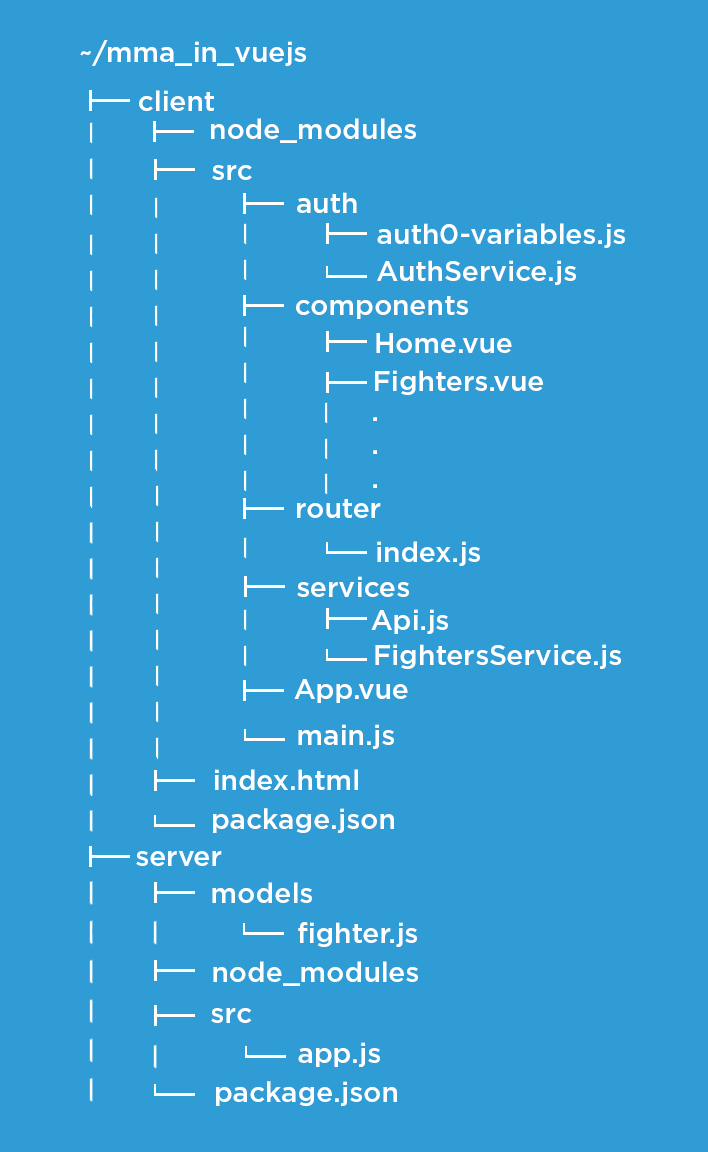
\includegraphics[scale=0.8]{kepek/mma_in_vue.jpeg}
\caption{A Vue.js projekt struktúrája}
\label{fig:vue_structure}
\end{figure}

A (\ref{fig:vue_structure}. ábra) a Vue.js webalkalmazáshoz tartozó projekt felépítését mutatja be. A szerver és a kliens részek külön mappákba kerültek, ez átláthatóbb struktúrát eredményez. A komponensek a "components" nevű mappában helyezkednek el. \cite{Vue könyv} \cite{Vue oldal} 
\Chapter{ReactJS implementáció}

CRUD műveletek megvalósítása

\begin{cpp}
constructor(props) {
    super(props);
    this.state = {
      fighters: []
    };
  }

  componentDidMount() {
    axios.get('/api/fighter')
      .then(res => {
        this.setState({ fighters: res.data });
      });
  }
\end{cpp}

A Fighters nevezetű komponensben a /components/Fighters.js fájlban a konstruktorban kell definiálnunk a „fighters” objektumot, a componentDidMount() nvevű függvény pedig az axios modulon keresztül egy http GET kérést küld a szervernek és a /api/fighter oldalról lekéri az aktuális harcosok listáját, majd beletölti a konstruktorban definiált fighters objektumba a response-ban (válasz) kapott adatokat.

Hasonló módon történik csak egy harcos lekérése is, ami a Show nevezetű komponens feladata:

\begin{cpp}
componentDidMount() {
    axios.get('/api/fighter/'+this.props.match.params.id)
      .then(res => {
        this.setState({ fighter: res.data });
      });
  }
\end{cpp}

Ebben az esetben szükséges van még a harcos id-jára is, amit a program az URL cím paraméteréből olvas ki. A konstruktorban pedig egy „fighter” objektumot kell megadni.

\begin{cpp}
this.state = { fighter: {} };
\end{cpp}

Új harcos létrehozását a Create nevezetű komponens végzi el:

\begin{cpp}
constructor() {
    super();
    this.state = {
      name: ' ',
      nickname: ' '
    };}
\end{cpp}

A konstruktorban definiálnunk kell a mezőket üres sztring-ekként. Majd a tényleges létrehozás a harcos adatait kérő form onSubmit={this.onSubmit} hatására hívódik meg a POST kérés a szerver felé.

\begin{cpp}
onSubmit = (e) => {
    e.preventDefault();
    const { name, nickname} = this.state;
    axios.post('/api/fighter', { name, nickname })
      .then((result) => {
        this.props.history.push("/fighters")
      }); }
\end{cpp}

Az axios modul segítségével egy HTTP POST kérést küldünk el a szerver felé a megfelelő paraméterek megadásával, majd ha sikeres a létrehozás, a program visszairányítja a felhasználót a /fighters oldalra.

Egy harcos adatainak a frissítéséhez szintén a form onSubmit={this.onSubmit} eseményére van szükségünk.

\begin{cpp}
onSubmit = (e) => {
    e.preventDefault();
    const { name, nickname } = this.state.fighter;
    axios.put('/api/fighter/'+this.props.match.params.id, { name, 
    nickname })
      .then((result) => {
        this.props.history.push("/fighters")
      });}
\end{cpp}

Az axios modul segítségével a program egy HTTP PUT kérést küld a szervernek a megfelelő paraméterekkel, majd a frissítés után visszairányítja a felhasználót a /fighters oldalra.

\begin{cpp}
delete(id){
    axios.delete('/api/fighter/'+id)
      .then((result) => {
        this.props.history.push("/fighters")
      });}
\end{cpp}

Egy harcos törléséhez pedig a delete() függvény meghívására van szükség, amit egy <button> gomb onClick eseményének meghívásával érhetünk el:

\begin{cpp}
<button class="btn btn-danger" onClick={this.delete.bind(this, 
this.state.fighter._id)}>Delete</button>
\end{cpp}

A delete() nevű függvénynek átadjuk a harcos id-ját majd az axios modulon keresztül egy HTTP DELETE kérést küldünk a szervernek, ha a program végrehajtotta a törlést, akkor visszairányít a /fighters oldalra.

\Section{Routing}

Az oldalak közötti routing az index.js nevű fájlban van megvalósítva:

\begin{cpp}
<Router history={history}>
	<div>
		<Route path='/edit/:id' component={Edit} />
        <Route path='/create' component={Create} />
        <Route path='/show/:id' component={Show} />
	</div>
</Router>
\end{cpp}

A path-nál kell megadnunk az URL címet, mellette a component-el adjuk meg, hogy arra a címre navigálva melyik komponensben definiált adatokat kell megjelenítenünk.

\Section{Form validáció}

A form validáláshoz a Create komponensben a konstruktorban definiált mezők mellett a következőket kell megadnunk:

\begin{cpp}
this.state = {
      name: ' ',
      nickname: ' ',
      formErrors: {name: ' ', weightclasses: ' '},
      nameValid: false,
      wecValid: false,
      formValid: false
};
\end{cpp}

A formErrors-ban a validálni kívánt mezőket kell definiálni, alapvetően a nameValid és wecValid változó értékét false-ra (hamis) állítjuk, így a formValid változó értéke is hamis lesz.

\begin{cpp}
validateField(fieldName, value) {
	let fieldValidationErrors = this.state.formErrors;
    let nameValid = this.state.nameValid;
    let wecValid = this.state.wecValid;
    switch(fieldName) {
    case 'name':
   	  nameValid = value.length >= 3;
      fieldValidationErrors.name = nameValid ? '': 'value is too short';
      break;
    case 'weightclasses':
      wecValid = value.toString().trim().length;
      fieldValidationErrors.weightclass = wecValid ? '' : ' is required';
      break;
      default:
      break; }
    this.setState({formErrors: fieldValidationErrors,
                    nameValid: nameValid,
                    wecValid: wecValid
                  }, this.validateForm);
}
\end{cpp}

A validateField() nevű függvényben definiálnunk kell pár változót, amik a kontruktorban megadott változók értékeit veszik fel.

Ezután egy switch-case szerkezetben megadhatjuk, hogy melyik esetben milyen hibaüzenetet adjon a program. 
A „name” mező esetében akkor lesz valid (érvényes) a mező, ha beírt érték hossza nagyobb, vagy egyenlő, mint 3. Tehát 3, vagy több karakteres name mező esetében a nameValid változó értéke true lesz, ellenkező esetben meghatározhatjuk a kiírandó hibaüzenetet.

A „weightclass” mező esetében ha a felhasználó beleír valamit a mezőbe, majd kitörli azt, akkor megjelenítődik a hibaüzenet.
A rekord mező esetében:

\begin{cpp}
case 'record':
	recValid = value.match(/^([0-9]+)-([0-9]+)-([0-9]+)$/i);
    fieldValidationErrors.record = recValid ? '': ' must be in 
    Wins-Draws-Losses form';
    break;
\end{cpp}

A felhasználó a rekordot csak győzelem-döntetlen-vereség formájában adhatja meg.

A this.setState rész fieldValidationErrors objektumot beletölti a formErrors objektumba, a mezők változóiba pedig a mezők érvényességének aktuális állapotát, majd meghívja a validateForm() függvényt.

\begin{cpp}
validateForm() {
 this.setState({formValid: this.state.nameValid && this.state.wecValid});
}
\end{cpp}

A függvény leellenőrzi, hogy érvényesek-e a mezők értékei és ha igen, akkor a form is érvényes lesz, tehát a formValid változó true értéket fog felvenni.

A form „Submit” neveztű gombja pedig mindaddig letiltásra kerül, ameddig a form nem érvényes.

\begin{cpp}
<button type="submit" disabled={!this.state.formValid} 
class="btn btn-default">Submit</button>
\end{cpp}

Ha a felhasználó beleír valamit a form-ba, a hibaüzenetek még nem fognak megjelenni mert még nem frissítjük az állapotát az input mezőnek, emiatt hozzákell adnunk az alábbi kódot a mezők input-jához.

\begin{cpp}
onChange={this.handleUserInput}
\end{cpp}

Ez a mező értékének változásakor meghívja a handleUserInput nevű függvényt, ami eltárolja egy konstansban a mező nevét, és egy másik konstansban a mező értékét, majd beállítja mezőnek az értéket és meghívja a validateField(fieldName, value) függvényt, aminek átadja a mező nevét és értékét, így a függvény az adott case-hez (eset) ugrik és eldönti, hogy a value (érték) alapján valid-e az adott mező, vagy nem.

Ha nem valid, akkor az aktuális mező hibaüzenetét elmenti a „formErrors” nevű objektumba.

\begin{cpp}
handleUserInput = (e) => {
    const name = e.target.name;
    const value = e.target.value;
    this.setState({[name]: value},
                  () => { this.validateField(name, value) }); }
\end{cpp}

A hibaüzeneteket a form tetején egy panel-ban jelenítjük meg:

\begin{cpp}
<div className="panel panel-default">
	<FormErrors formErrors={this.state.formErrors} />
</div>
\end{cpp}

A nem érvényes mezők piros szegéllyel való megjelenítéséért pedig az alábbi kód felel:

\begin{cpp}
<div className=
	{`form-group ${this.errorClass(this.state.formErrors.name)}`}>
<label htmlFor="name">Name*</label>
\end{cpp}

Ez meghívja az errorClass() nevű függvényt a mező aktuális hibaüzenetével, így az érvénytelen mezők a „has-error” class-t kapják meg, tehát piros szegélyük lesz.

\begin{cpp}
errorClass(error) {
    return(error.length === 0 ? '' : 'has-error');}
\end{cpp}

Szükség van még a FormErrors nevű osztályra, amit importálnunk kell:

\begin{cpp}
import { FormErrors } from './FormErrors';
\end{cpp}

A FormErrors osztály pedig így néz ki:

\begin{cpp}
export const FormErrors = ({formErrors}) =>
  <div className='formErrors'>
    {Object.keys(formErrors).map((fieldName, i) => {
      if(formErrors[fieldName].length > 0){
        return (
          <p key={i}>{fieldName} {formErrors[fieldName]}</p>
        )        
      } else {
        return ' ';
      } })} </div>
\end{cpp}

Ez a kód végigmegy a formErrors objektumon és megjeleníti az azon belül található hibákat.

\Section{A harcosok táblázatának szűrése}

A Fighters.js nevű komponens konstruktorában a CRUD műveleteknél látott „fighters” objektumon kívül egy „filterText” nevű változót kell definiálni egy üres sztring-ként.

\begin{cpp}
constructor(props) {
    super(props);
    this.state = {
      filterText: '',
      fighters: []
    };
  }
\end{cpp}

Ezenkívül az updateSearch() nevű függvény frissíti a filterText mező aktuális állapotát.

\begin{cpp}
updateSearch(event){
    this.setState({filterText: event.target.value.substr(0,20)}); }
\end{cpp}

A megjelenítendő adatok a render() függvényen belül találhatók, itt meg kell adnunk egy új objektumot, ez esetben a „filteredFighters” nevű objektumot, ami a fighters objektumra hívja meg a filter direktívát, ami megnézi minden fighter-re, hogy a name mezője értékének kisbetűssé alakított változata tartalmazza-e a filterText mező értékének kisbetűssé alakított változatát és ha igen, akkor benne hagyja a filteredFighters objektumban, ha nem, akkor kiveszi belőle. Ha az alábbi kifejezés egyenlő -1-el, akkor amelyik nem tartalmazza, az kikerül az objektumból, így a táblázatból is.

\begin{cpp}
render() {
 let filteredFighters = this.state.fighters.filter(
  (fighter) => {
   return fighter.name.toLowerCase()
   .indexOf(this.state.filterText.toLowerCase()) !== -1;
 }
);
\end{cpp}

A táblázaton belül létre kell hozni egy beviteli mezőt, aminek értékét a konstruktorban definiált filterText-re állítjuk be. A filterText mező értékének változásakor meghívja az
updateSearch() függvényt a mező aktuális állapotával, így az mindig beállítja neki az újabb állapotot egészen a 20. karakterig.

\begin{cpp}
return (
  <div className="ftable">
    <div className="search">
      <input type="text" class="searchbar" value={this.state.filterText} 					   onChange={this.updateSearch.bind(this)} placeholder="Search fighters...">
      </input>
  </div>
\end{cpp}

Az alábbi kód a táblázat <tbody></tbody> tag-jei között itrál végig a filteredFighters objektumon, és megjeleníti a harcosok adatait.

\begin{cpp}
<tbody>
{filteredFighters.map(fighter =>
<tr>
	<td>{fighter.name}</td>
	<td>{fighter.nationality}</td>
</tr>
)}
</tbody>
\end{cpp}


\Section{Projekt struktúra}

\begin{figure}[htb]
\centering
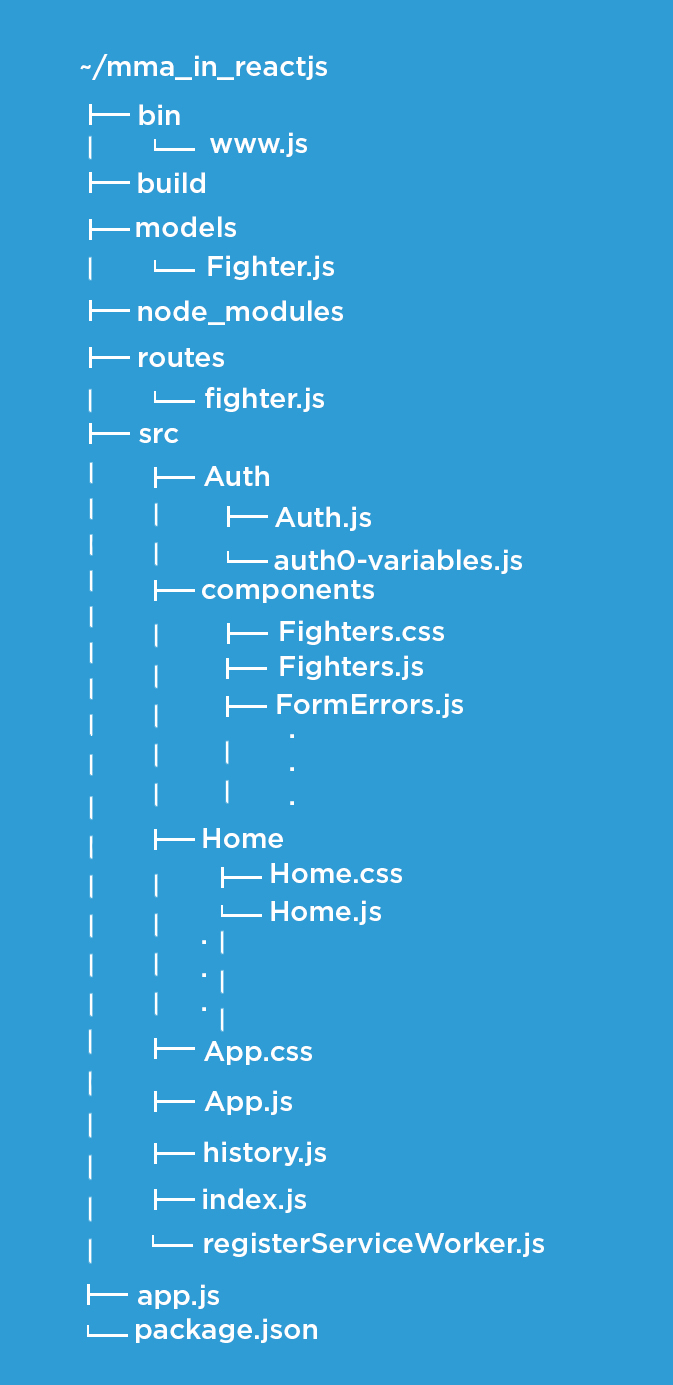
\includegraphics[scale=0.7]{kepek/mma_in_reactjs.jpeg}
\caption{A ReactJS projekt struktúrája}
\label{fig:reactjs_structure}
\end{figure}


\newpage
\Section{Auth0 szervíz}

\begin{cpp}
handleAuthentication() {
    this.auth0.parseHash((err, authResult) => {
      if (authResult && authResult.accessToken && authResult.idToken) {
        this.setSession(authResult);
        history.replace('/home');
      } else if (err) {
        history.replace('/home');
        console.log(err);
        alert(`Error: ${err.error}. Check the console for further details.`);
      }
    });
  }

  setSession(authResult) {
    // Set the time that the access token will expire at
    let expiresAt = JSON.stringify(
      authResult.expiresIn * 1000 + new Date().getTime()
    );
    localStorage.setItem('access_token', authResult.accessToken);
    localStorage.setItem('id_token', authResult.idToken);
    localStorage.setItem('expires_at', expiresAt);
    // navigate to the home route
    history.replace('/home');
  }

  getAccessToken() {
    const accessToken = localStorage.getItem('access_token');
    if (!accessToken) {
      throw new Error('No access token found');
    }
    return accessToken;
  }

  getProfile(cb) {
    let accessToken = this.getAccessToken();
    this.auth0.client.userInfo(accessToken, (err, profile) => {
      if (profile) {
        this.userProfile = profile;
      }
      cb(err, profile);
    });
  }

  logout() {
    // Clear access token and ID token from local storage
    localStorage.removeItem('access_token');
    localStorage.removeItem('id_token');
    localStorage.removeItem('expires_at');
    this.userProfile = null;
    // navigate to the home route
    history.replace('/home');
  }

  isAuthenticated() {
    // Check whether the current time is past the 
    // access token's expiry time
    let expiresAt = JSON.parse(localStorage.getItem('expires_at'));
    return new Date().getTime() < expiresAt;
  }
\end{cpp}

\Chapter{Auth0 szervíz}

Az Auth0 egy olyan platform, amit a fejlesztők használhatnak arra, hogy alkalmazásaikba autentikációt és autorizációt ültessenek. Támogatja a legelterjedtebb keretrendszereket és technológiákat, dokumentációja átlátható. Továbbá egy folyamatosan fejlődő, innovatív rendszer. \cite{Auth0}

Az egyes keretrendszerek programjaiban való alkalmazása a következő módon történik: (home.component.html fájl)

\subsubsection{Angular 2 esetében:}

\begin{cpp}
<h4 *ngIf="auth.isAuthenticated()">
    <div>
   	<a [routerLink]="['/fighter-create']">ADD NEW FIGHTER</a>
   	</div>
</h4>
<h4 *ngIf="!auth.isAuthenticated()">
  You are not logged in! Please 
  <a (click)="auth.login()">Log In</a> to continue.
</h4>
\end{cpp}

Az fenti kód az "*ngIf" direktíva használatával meghívja az "auth" "isAuthenticated()" függvényét, amely leellenőrzi, hogy a felhasználó be van e jelentkezve és ha igen, akkor megjeleníti az "ADD NEW FIGHTER" nevű linket. Ha a felhasználó nincs bejelentkezve, akkor a "You are not logged in" üzenet és a "Please Log In to continue" üzenet jelenik meg, ahol a "Log In" egy gomb, ami meghívja az "auth" "login()" függvényét.

Az Auth0 szerviz használatához szükség van egy felhasználói fiók létrehozására az Auth0 hivatalos weboldalán, majd a megfelelő keretrendszer kiválasztása után az adott keretrendszerre nézve szükséges végrehajtani a leírt lépéseket, hogy az alkalmazásunkba integrálhassuk a szervizt.

A "home.component.ts" fájlban szükséges importálni a következő parancsot:
\begin{cpp}
import { AuthService } from './../auth/auth.service';
\end{cpp}

Továbbá a konstruktorban definiálni az "auth"-ot, mint az előbb beimportált\\ "AuthService" nevű szervizt:
\begin{cpp}
export class HomeComponent implements OnInit {

  constructor(public auth: AuthService) { }
  ngOnInit() {
  }
}
\end{cpp}

A felhasználó azonosításától függően megjeleníteni kívánt tartalom kódja a többi keretrendszer esetében is hasonló elven működik. Használata direktívákkal történik. Minden keretrendszerhez megtalálható a megfelelő dokumentáció az Auth0 hivatalos oldalán. \cite{Auth0}
\Chapter{Keretrendszerek összehasonlítása}

\begin{tabular}{|p{2,3cm}|p{2,5cm}|p{2,95cm}|p{2,8cm}|p{2,65cm}|}
\hline
\textbf{} & \textbf{AngularJS} & \textbf{Angular 2} & \textbf{React.js} & \textbf{Vue.js} \\
\hline
\textbf{Fejlesztő} & Google & Google & Facebook, Instagram & JavaScript könyvtár \\
\hline
\textbf{Github} & commit: 8629, contributor: 1603 & commit: 9009, contributor: 540 & commit: 9425, contributor: 1139 & commit: 2378, contributor: 159 \\
\hline
\textbf{Google találat} & 118 millió  & 103 millió & 180 millió & 23 millió 400 ezer \\
\hline
\textbf{Méret} & 1239 KB, min: 165 KB & 1044 KB, min: 566 KB & 45 KB, min: 6 KB & 272 KB, min: 84 KB \\
\hline
\textbf{Elérhető irodalom} & angularjs.org & angular.io & reactjs.org & vuejs.org \\
\hline
\textbf{Megjelenés Verzió} & 2010.október 1.6.6 & 2014.szeptember 2.0.0 & 2013.március 16.2.0 & 2014.február 2.5.3 \\
\hline
\textbf{Típus} & JavaScript keretrendszer & JavaScript keretrendszer & JavaScript könyvtár & JavaScript keretrendszer \\
\hline
\end{tabular}
\\
\SubSection{Form validáció}
\subsubsection{AngularJS:} "ng-class" és css class-ok együttes használata, direktívák használata a hibaüzenetek megjelenítéséhez (ng-show), egyszerűen megvalósítható. A "number" típusú mezők validálása a "min" és "max" direktívákkal minden további gond nélkül megoldható. Továbbá lehetőség van saját érvényesség ellenörző direktívák létrehozására is. \\
\subsubsection{Angular 2:} Az "*ngIf" és "ngModel" direktívák használatával egyszerűen megvalósítható. Lehetőség van továbbá úgynevezett saját érvényesség ellenőrző direktívák létrehozására, ahol meg lehet határozni, hogy mit ne fogadjon el, esetleg mit fogadjon el a program lehetséges input-ként. A "number" típusú mezők validálása csak külön modullal vagy saját érvényesség ellenőrző direktíva létrehozásával érhető el, amely néha kényelmetlenségeket okozhat. Viszont a különböző mezőknél történő saját hibaüzenet megadásának lehetősége, és az azok közötti automatikus váltás kárpótol emiatt.\\
\subsubsection{Vue.js:} A "vee-validate" modul telepítése szükséges hozzá, elérhető 20 validációs szabály, mint például "alpha\_spaces", amely azt hivatott ellenőrizni, hogy az adott input mező tartalmaz-e szóközt, ha igen, akkor érvényes a mező. Jól használható név mezők esetében, ahol az a fontos, hogy ne lehessen a mezőben numerikus karakter, de lehessen benne szóköz. A validációs üzenetek beépítettek, de lehetőség van a változtatásukra. Személy szerint ebben a keretrendszerben használható fentebb említett modul miatt ezt a megoldást találtam a legkényelmesebbnek a rendelkezésre álló szabályok sokszerűsége miatt.\\
\subsubsection{React.js:} A form validáció implementálása ebben a keretrendszerben volt a legnehezebb és a legtöbb időt ez vette igénybe, lévén, hogy nincs kétirányú adatkötés, így különböző validációs funkciókat kellett létrehozni a kívánt eredmény eléréséhez, továbbá ennél a megoldásnál a validációs hibaüzenetek csak a kitöltendő form felett lévő panel-ban jelennek meg.\\
\Chapter{Összegzés}

A dolgozat első részében az MVC keretrendszerről, a JavaScript és ECMAScript közötti különbségről, a verziókról és történelmi áttekintésről volt szó. Ezután az a JavaScript keretrendszerek előnyeit, hátrányait mutattam be. Ezt követően a mintaalkalmazások specifikációja található meg.
A dolgozat fő témája a keretrendszerek több szempontból való összehasonlítása. Ezek a szempontok a CRUD műveletek megvalósítása, template-k és a weboldalak közötti routing működése, szűrők és direktívák használata, form validáció, valamint bejelentkezés és regisztráció. 
A négy webalkalmazás AngularJS, Angular 2, Vue.js, és React.js keretrendszerekben készült el. A backend részhez a MongoDB nevű programot használtam az adatok tárolására, a Node.js-t a szerver megvalósításához. A weboldalak az MMA harcosokkal foglalkoznak (MMA Fighters).
\\Véleményem szerint az AngularJS keretrendszer a legkönnyebben megérthető egy web-es oldalak világában és technológiáiban nem teljesen jártas ember számára is, a tesztelése a különböző részeknek egyszerűen megoldható és a kétirányú adatkötés használata megkönnyíti a fejlesztést. Ezenfelül az Angular 2-nél és a React.js-nél a komponensek generálásának lehetősége jelentősen lecsökkentette a fejlesztési időt. A React.js használatának megtanulása több időt és erőfeszítést igényel, mindezek mellett jobb megoldás lehet egy nagyobb, komplexebb alkalmazás elkészítéséhez. A Vue.js egy gyors alternatíva, amely ezeknek a keretrendszereknek a legjobb tulajdonságait ötvözi, olyanokat, mint az AngularJS-ben megismert kétirányú adatkötés, JSX támogatás, vagy szerver-oldali renderelés.
Az Auth0 szerviz mindegyik keretrendszerhez megtalálható, dokumentációjuk átlátható, követhető. 

További tervek, ötletek \\
A alkalmazások továbbfejlesztése, kibővítése újabb funkciókkal. Tervek között szerepel a képfeltöltés funkciójának megvalósítása, saját Auth0 szerviz bejelentkezési form létrehozása, admin és vendég felület hozzáadása.

Mindegyik keretrendszernek és technológiának vannak előnyei és hátrányai, amikkel a fejlesztők, és a cégek tisztában vannak, ennek ellenére egy jó lehetőség belelátni ezeknek a technológiáknak a működésébe, használatuknak rejtélyeibe és mindenképpen előny többféle keretrendszer elemeinek és működésének megismerése.


\Chapter{Summary}

In my thesis i compared the most popular JavaScript frameworks. In the first part i demonstrated that what is the MVC framework, what is the difference between JavaScript and ECMAScript, there was a part of the versions and lastly a historical overview. Thereafter an overview of JavaScript technologies.\\
The main subject was to compare the frameworks and libraries in a few aspects. Those are the CRUD operations, templates, routing, filters, directives, form validation, and also login with an option to sign up.
The four web applications what i implemented are AngularJS, Angular 2, Vue.js, and React.js. The MongoDB database and the Node.js server provides the backend functionalities. These web applications are deal with MMA Fighters. There is an option to log in or sign up, to add a new fighter, to see the fighters who are stored in the database, to filter the table of fighters, to edit the fighter's details and to delete the fighters.\\ The AngularJS framework is a very good option to develop web applications, and it is not really hard to learn for those who are not proficient in the web pages world. Maintaining and testing the separated parts is really easy to handle. The two-way data binding is simplify the development phase. In Angular 2, React.js, and Vue.js the option to generate the components and services with their CLI-s is very handy. These frameworks are well-known and very popular in firms. The Vue.js is a framework which is combine the advantages of the other frameworks. It is a fast alternative, and growing quickly. 
Because of the JSX and ES6 elements the React.js is need more time and efforts to learn how to use the library.\\
The Auth0 platform is a powerful and popular solution to integrate into any web application. It has a well-founded documentation, and support the most popular frameworks and API-s.\\
My further plans and ideas to work on in these applications are to add new functions, like image uploading for the fighter's image field, create a custom login and signup form with Auth0, and also to create an administrator and guest interface.\\
Each one of these frameworks has advantages over the others, and also has disadvantages as well, which the developers or firms could accept.
In my opinion it is a good opportunity to choose from this big lineup of technologies and take time to meet and learn them. 






\begin{thebibliography}{x}
\addcontentsline{toc}{chapter}{\bibname}
\bibitem{PlainTeX} Bujdosó Gyöngyi, Fazekas Attila: {\em\TeX\ kezdõlépések}, Tertia Kiadó, Budapest, 1997.
\bibitem{Hazy2005} Házy Attila: {\em Lineáris függvényegyenletek megoldása számítógéppel}, Doktoranduszok fóruma 2005, Miskolc, 2005. november 9., Gépészmérnöki Kar szekciókiadványa, Miskolc, ME ITTC, 2006., 108--113.
\bibitem{LaTeX} Hettl, Mayer, Szabó: {\em \LaTeX\ kézikönyv}, Panem Könyvkiadó, Budapest, 2004.
\bibitem{Hohmeyer} M. E. Hohmeyer, B. A. Barsky: Rational continuity: parametric, geometric and Frenet frame
continuity of rational curves, {\em ACM Transactions on Graphics}, \textbf{8} (1989), 335--359.
\bibitem{TeX_Catalogue} \TeX\ Catalogue, {\ttfamily www.ctan.org/tex-archive/help/Catalogue/catalogue.html} 
\end{thebibliography}

\newpage


%Az �sszefoglal� fejezet
\chapter*{Adathordoz� haszn�lati �tmutat�}
\addcontentsline{toc}{chapter}{Adathordoz� haszn�lati �tmutat�}

Ebben a fejezetben kell megadnunk, hogy a szakdolgozathoz mell�kelt adathordoz�t (pl. CD) hogyan lehet el�rni, milyen struktur�t k�vet. Minimum 1 maximum 4 oldal a terjedelem. Lehet benne t�bb alszakasz is. A fejezet c�me nem m�dos�that�, hasonl�an a k�vetkez� r�szhez (Irodalomjegyz�k).


\end{document}
